\documentclass[12pt,a4paper]{report}

% Packages
\usepackage{graphicx}
\usepackage{amsmath}
\usepackage{hyperref}
\usepackage{setspace}
\usepackage{float}
\usepackage{geometry}
\usepackage{enumitem}


% Title and Author (adjust the spacing as needed)
\title{\LARGE \textbf{PROJECT TITLE}}
\author{}
\date{\large On: \today}

% Begin Document
\begin{document}

% Title Page
\makeatletter
\begin{titlepage}
    \centering
    \vspace*{1cm}
       { 
\includegraphics[width=6cm]{figs/logo.jpg}}\\[1cm]

    {\LARGE \textbf{EXPERIMENT-1}}\\[1cm]
    
    
    
    \textbf{Instructor: }{Prof. Gajendranath Chowdary}\\[1cm]
    
    \textbf{Written By:}\\{RONGALI CHARAN - EE24BTECH11052\\ ANKIT JAINAR - EE24BTECH11004}\\[1cm]
    \date{\large Date Last Edited: \today}
    {\@date\\}
\end{titlepage}
\makeatother
% Abstract

\chapter*{Abstract}
\addcontentsline{toc}{chapter}{Abstract}
Lissajous figures, intricate patterns formed by the combination of two perpendicular sinusoidal signals, are frequently observed on oscilloscopes in physics and engineering laboratories. These figures provide valuable insights into phase relationships and frequency ratios between two signals. By varying the amplitude, frequency, and phase difference of the input signals, a wide variety of closed and open curves can be generated, each corresponding to specific mathematical relationships. Lissajous figures are particularly useful in signal analysis and calibration tasks, enabling precise comparisons of waveform characteristics.

The phenomenon is commonly demonstrated using a Cathode Ray Oscilloscope (CRO), where one signal is applied to the horizontal deflection plates and another to the vertical deflection plates. When the frequency ratio between the signals is rational, the resulting pattern is stable and periodic. Conversely, irrational ratios yield non-repeating, complex traces. These figures find applications in areas such as communication systems, control theory, and the visualization of harmonic motion.

Capturing one-time events on a CRO, such as transient signals or singular disturbances, requires the device to operate in storage mode or use an advanced digital oscilloscope capable of memory functions. This capability is essential in analyzing events like lightning surges, signal spikes, or transient faults in electronic circuits. Techniques such as trigger-based synchronization are employed to ensure that the fleeting event is displayed and recorded accurately. Advanced CROs also allow for the integration of digital storage, enabling further analysis and processing of captured data.

This paper explores the mathematical principles behind Lissajous figures, their practical implementation on CROs, and techniques for capturing one-time events. By bridging theoretical concepts with practical applications, it underscores the relevance of oscilloscopes in modern signal analysis and highlights their indispensability in both academic research and industrial diagnostics.


% Table of Contents
\tableofcontents



% List of Figures
\listoffigures

% Chapters
\chapter{Lissajous Figures}
\section{Set Up}

To set up the oscilloscope and function generator for observing and taking readings of Lissajous figures, follow these steps:

 \textbf{1. **Equipment Preparation:**}
\begin{itemize}
    \item Ensure you have a Cathode Ray Oscilloscope (CRO) and a Function Generator.
   \item Check that both devices are powered on and in working condition.
\end{itemize}
 \textbf{2. **Initial Oscilloscope Configuration:**}
\begin{itemize}
    \item Set the oscilloscope to `XY Mode`. This mode allows the horizontal and vertical inputs to be controlled independently by the respective signals.
   \item Connect the oscilloscope probes to the input terminals and ensure they are functioning correctly.
\end{itemize}

 \textbf{3. **Function Generator Setup:**}
\begin{itemize}
    \item Connect the first function generator to the horizontal input (X-axis) of the oscilloscope.
   \item Connect the second function generator to the vertical input (Y-axis) of the oscilloscope.
   \item Use coaxial cables or BNC connectors to ensure proper signal transmission.
\end{itemize}
 \textbf{4. **Signal Configuration:**}
\begin{itemize}
   \item  Set the desired frequency and amplitude on both chanels of function generator.
   \item Adjust the phase difference between the signals if required. The phase difference significantly affects the shape of the Lissajous figures.
   \item Ensure that at least one of the signals has a controllable phase shift.
\end{itemize}


 \textbf{5. **Observation and Recording:**}
 \begin{itemize}
    \item  Observe the Lissajous figures on the oscilloscope screen.
    \item  Fine-tune the amplitude, frequency, and phase settings to obtain the desired pattern.
    \item  Record the observed figures, noting the frequency ratio and phase difference for each pattern.
\end{itemize}
 \textbf{6. **Safety Checks:**}
 \begin{itemize}
    \item Ensure all connections are secure and there are no loose wires.
    \item  Avoid setting amplitudes too high, as this can damage the oscilloscope or function generator.
\end{itemize}
By following these steps, you can successfully generate and analyze Lissajous figures using the oscilloscope and function generator.

\section{CRO Graphs}
\subsection{One}
\subsubsection*{Wave Equations}
The two sine waves are represented as:
\[
V_1(t) = A_1 \sin(2 \pi f t + \phi_1)
\]
\[
V_2(t) = A_2 \sin(2 \pi f t + \phi_2)
\]
where:
\begin{itemize}
    \item \(A_1, A_2\) are the amplitudes of the two signals.
    \item \(f\) is the common frequency of both signals.
    \item \(\phi_1, \phi_2\) are the phase angles of the signals.
\end{itemize}

\subsubsection*{Observed CRO Patterns}
From the plots:
\begin{itemize}
    \item The sine wave in \textbf{Channel 1} is given by:
    \[
    V_1(t) = A \sin(2 \pi f t)
    \]
    \item The sine wave in \textbf{Channel 2} is given by:
    \[
    V_2(t) = A \sin(2 \pi f t)
    \]
    Here, the amplitudes (\(A\)) and frequencies (\(f\)) of both signals are identical, and the signals are perfectly in phase (\(\phi_1 = \phi_2\)).
\end{itemize}

\subsubsection*{Lissajous Figure in X-Y Mode}
When the signals are displayed in X-Y mode on the CRO, the parametric equations for the plot are:
\[
x(t) = V_1(t) = A \sin(2 \pi f t)
\]
\[
y(t) = V_2(t) = A \sin(2 \pi f t)
\]

Since \(V_1(t)\) and \(V_2(t)\) are perfectly in phase (\(\phi_1 = \phi_2\)), we have:
\[
y(t) = x(t)
\]

This produces a straight line in the Lissajous figure, where:
\[
y = x
\]
\subsubsection*{Conclusion}
The observed straight-line Lissajous figure confirms that:
\begin{itemize}
    \item The signals in Channel 1 and Channel 2 are in phase.
    \item Their frequencies and amplitudes are identical.
\end{itemize}
\subsubsection*{Figure of CRO Patterns}
\begin{figure}[H] % H forces the figure to be placed exactly here
    \centering
    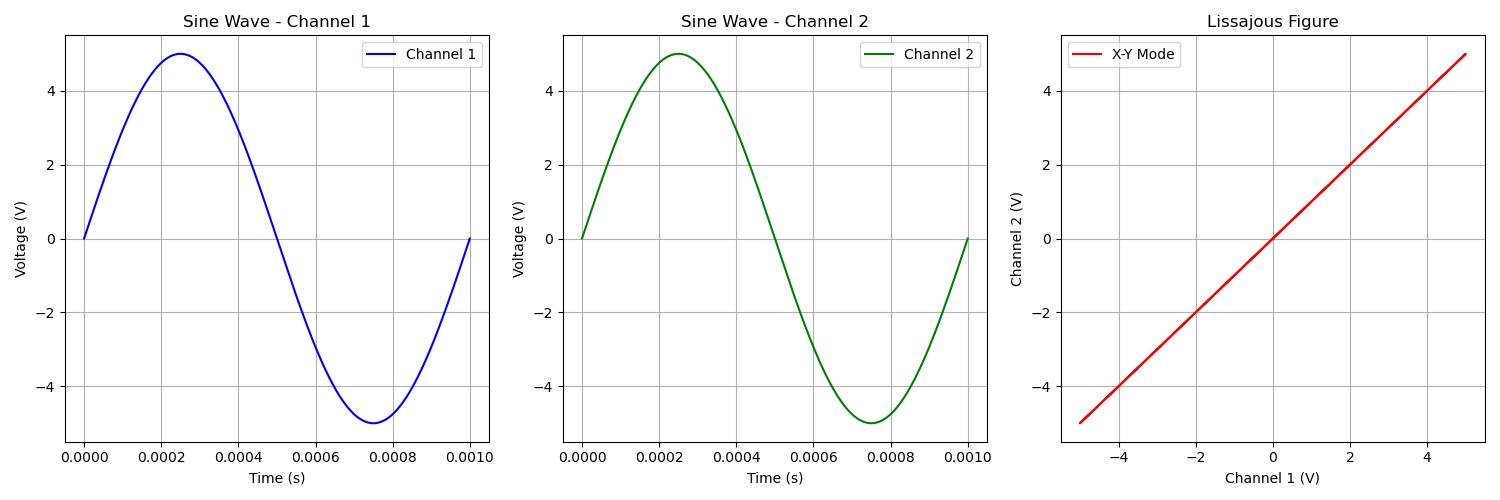
\includegraphics[width=\textwidth]{figs/1.jpg} % Replace "1.jpg" with your actual image filename
    \begin{minipage}[c]{0.48\textwidth}
        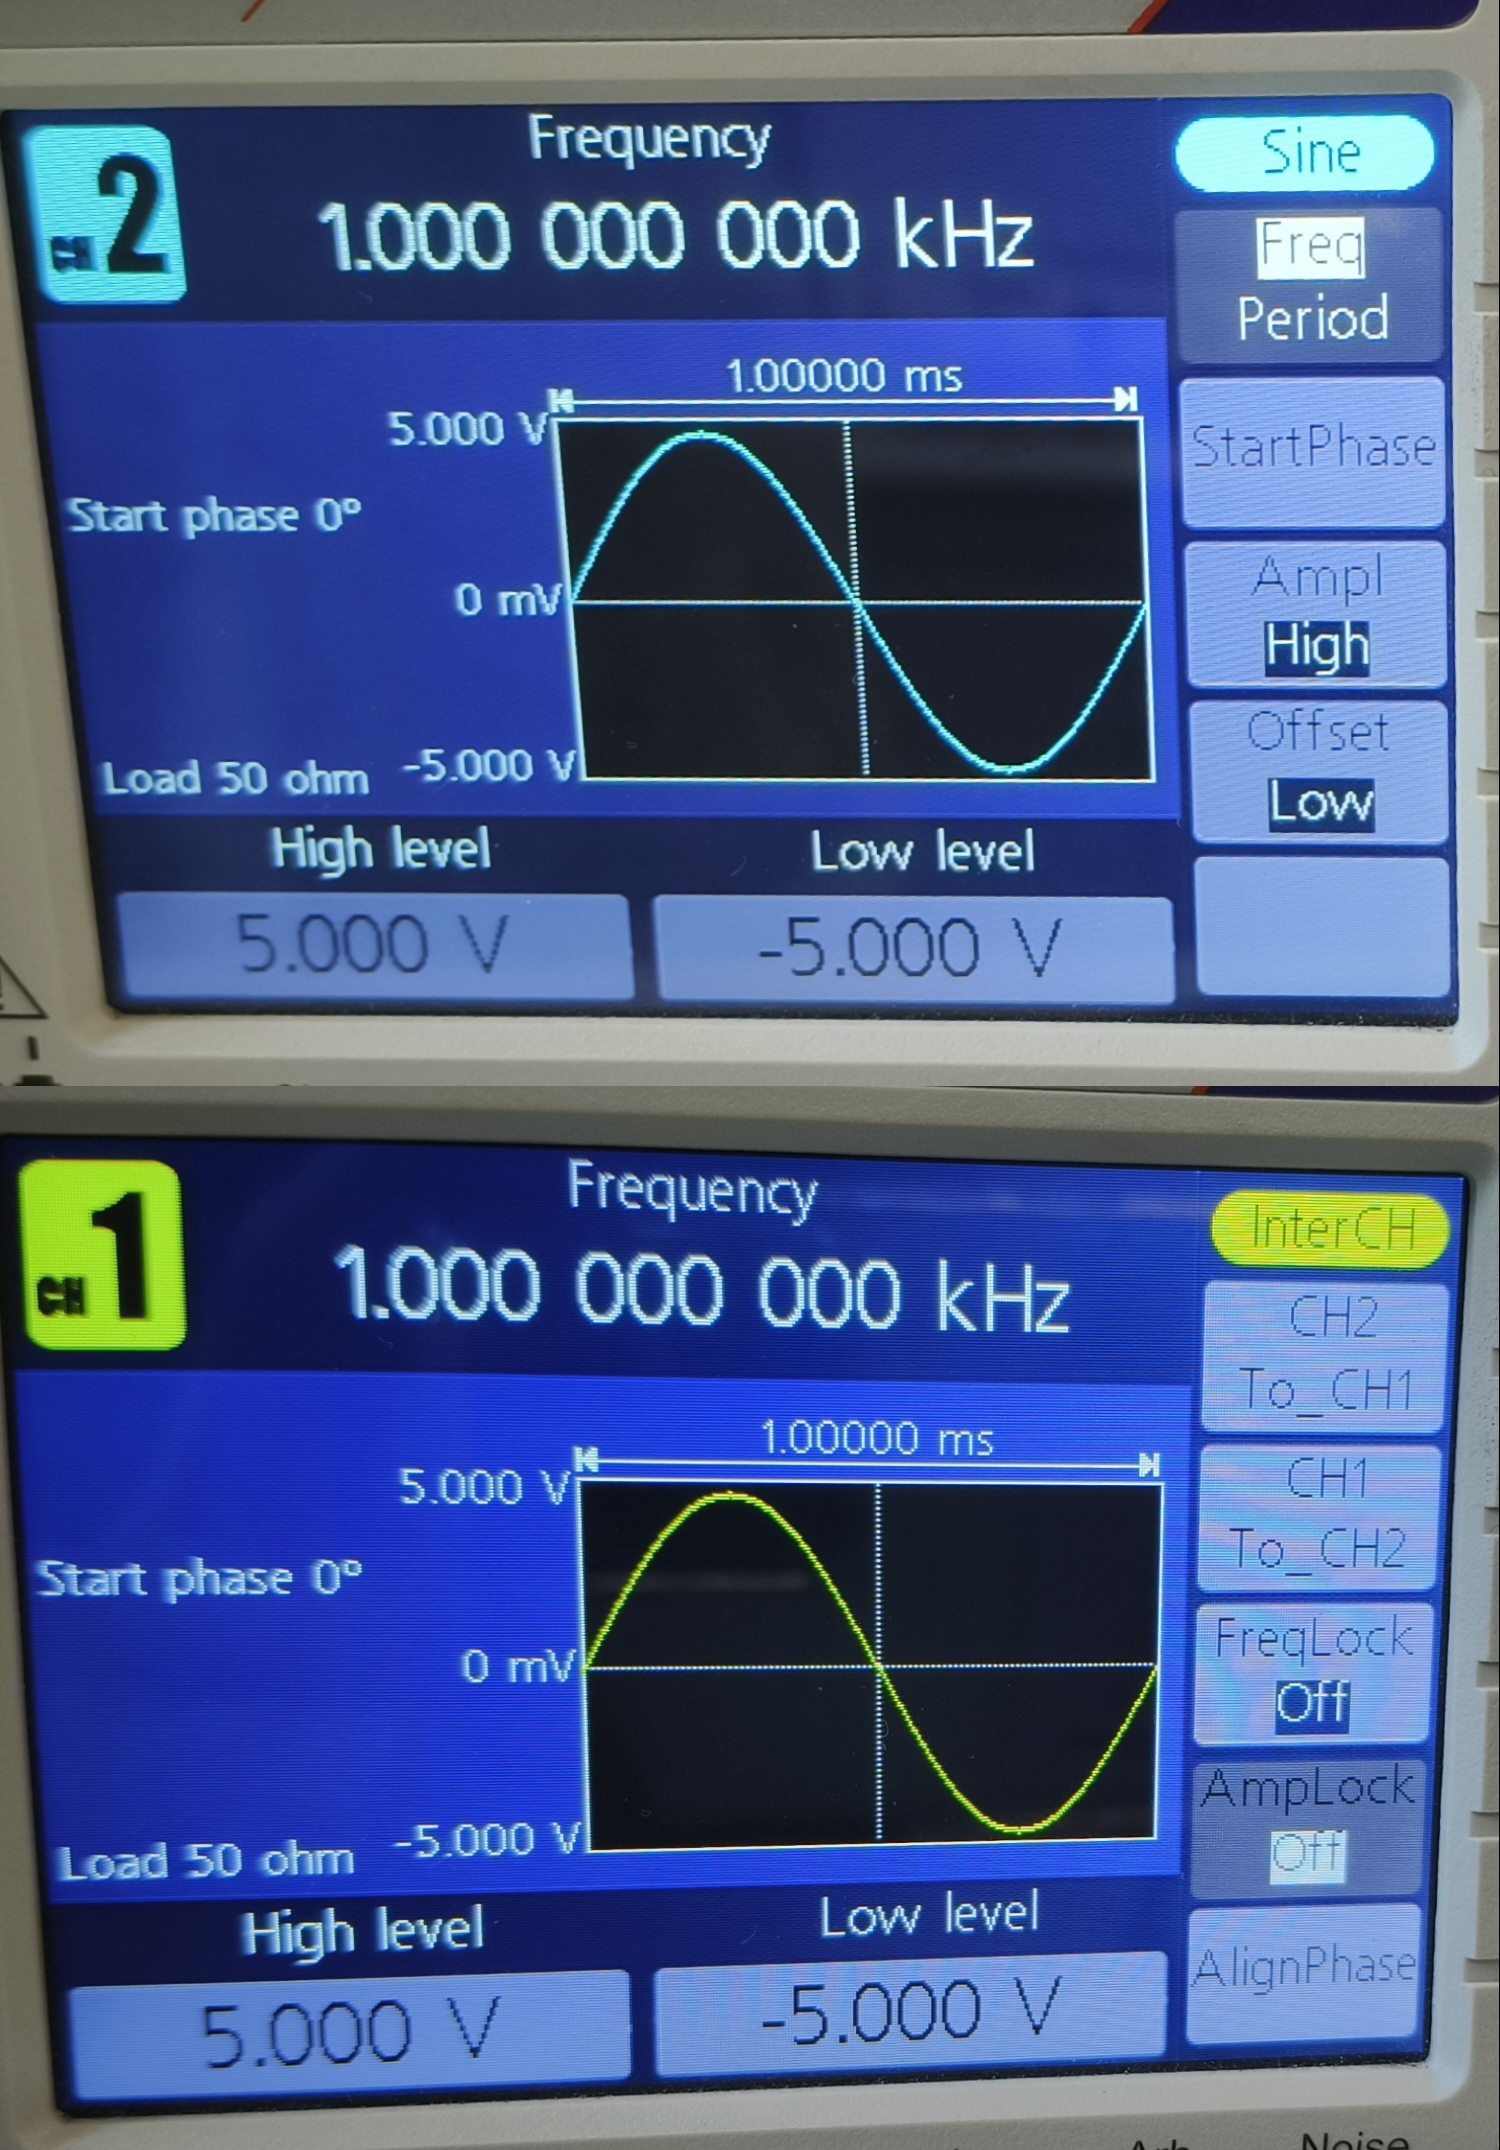
\includegraphics[width=\textwidth]{figs/1read.jpg} % Replace with the actual file name
        
    \end{minipage}
    \hfill
    \begin{minipage}[c]{0.48\textwidth}
        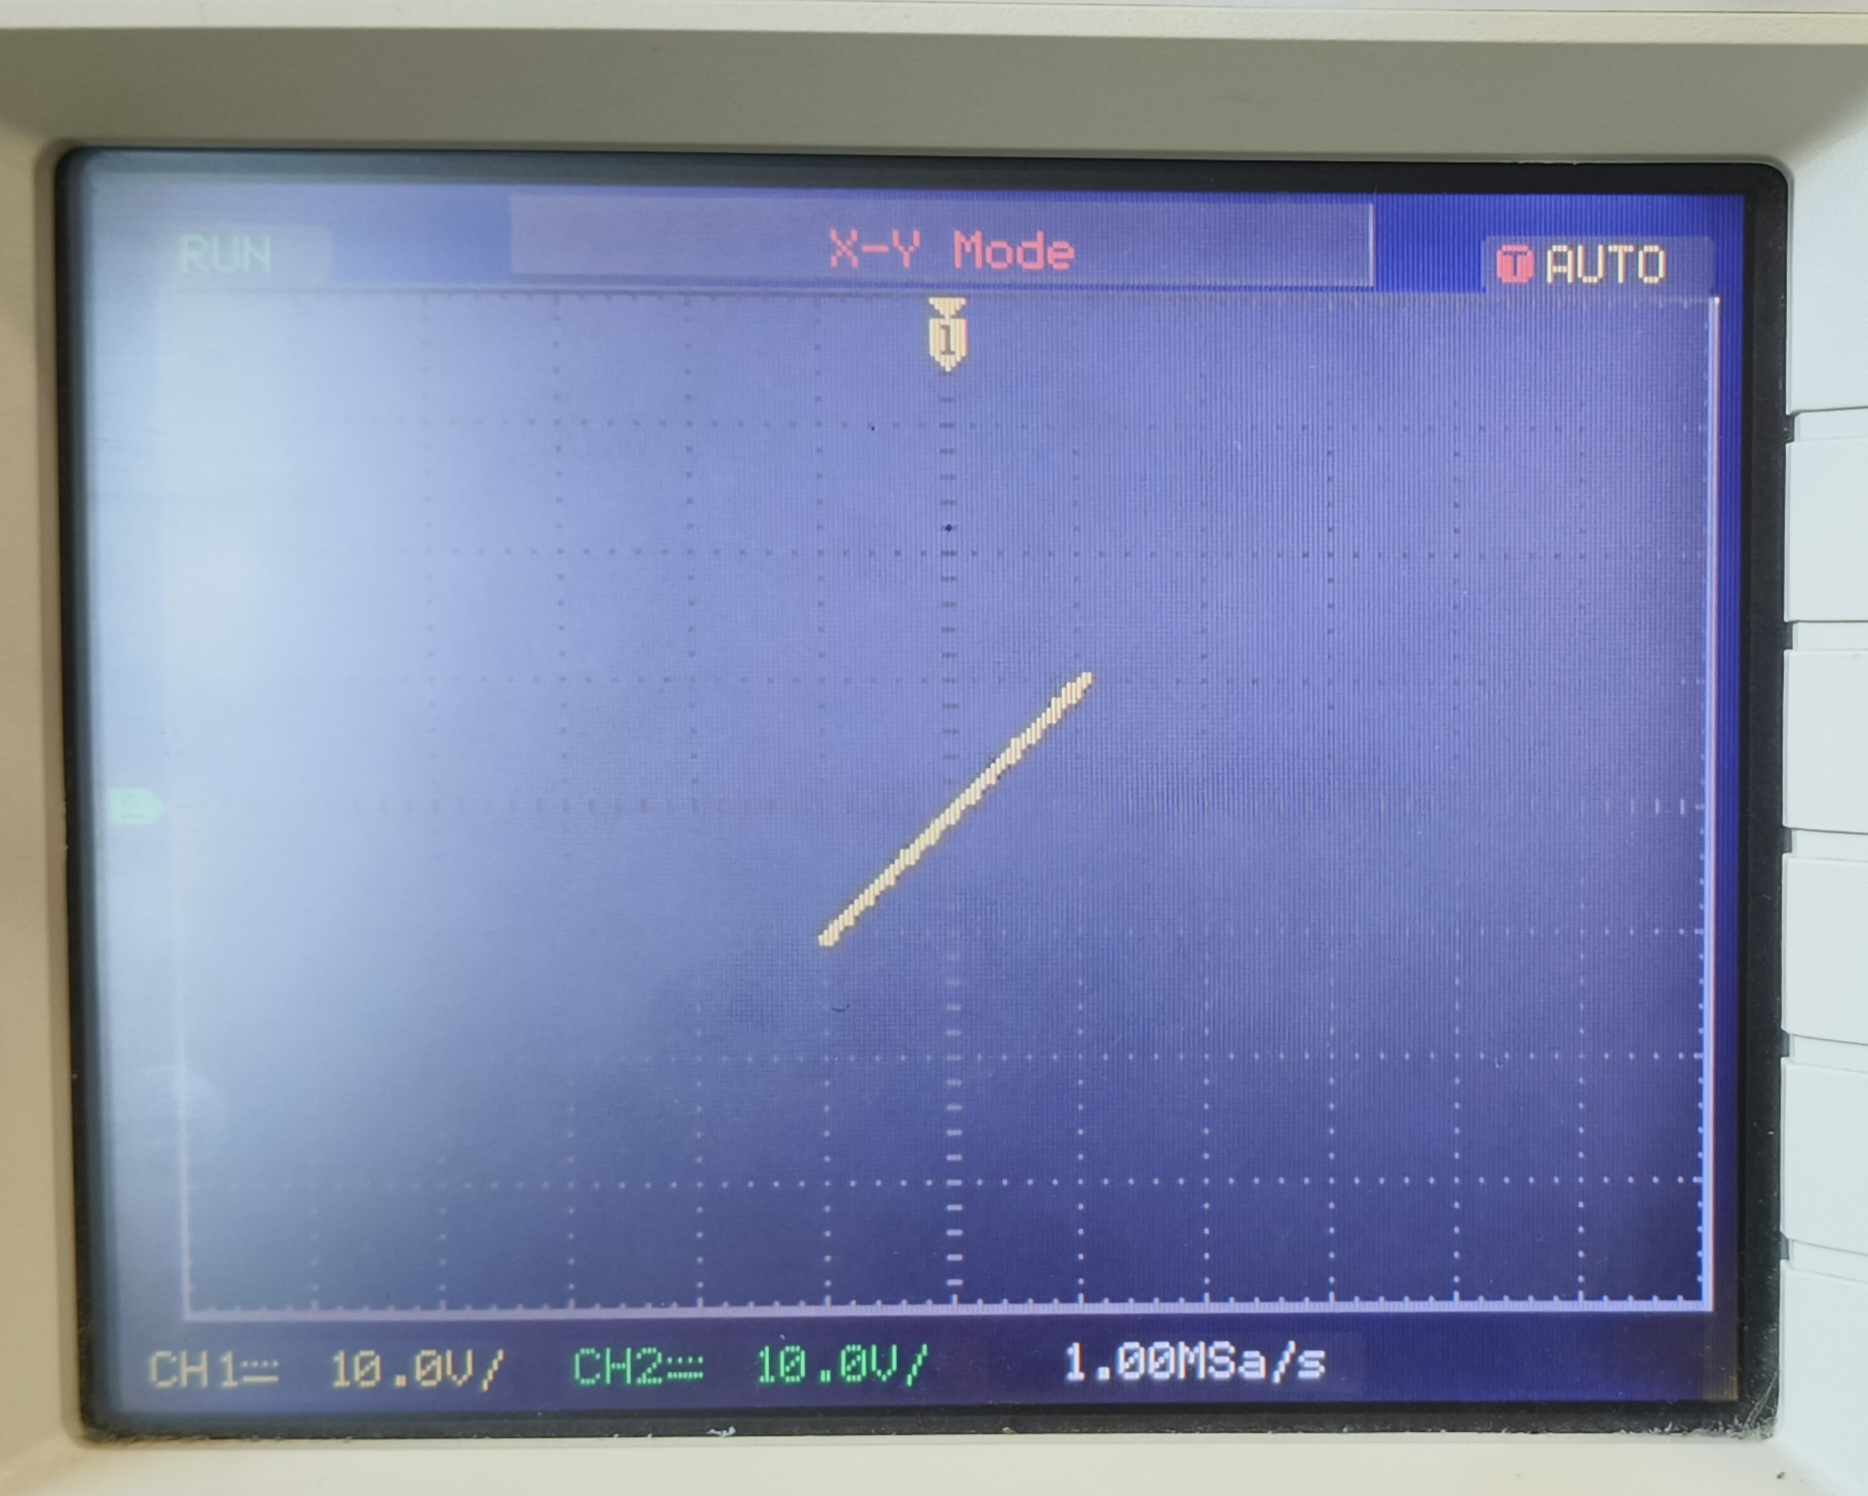
\includegraphics[width=\textwidth]{figs/1cro.jpg} % Replace with the actual file name
        
    \end{minipage}
    \caption{Graph 1}
    \label{fig:CRO-patterns}
\end{figure}
\subsection{Two}
The two sine waves are represented as:
\[
V_1(t) = A_1 \sin(2 \pi f_1 t + \phi_1)
\]
\[
V_2(t) = A_2 \sin(2 \pi f_2 t + \phi_2)
\]

\subsubsection*{Case 1: Same Frequency (\(f_1 = f_2 = f\))}
If the two signals have the same frequency, the resulting Lissajous figure depends on the phase difference (\( \Delta \phi = \phi_2 - \phi_1 \)).

\begin{itemize}
    \item \(\Delta \phi = 0\): Signals are in phase, and the figure is a straight line with a positive slope.
    \item \(\Delta \phi = \pi/2\): Signals are \(90^\circ\) out of phase, producing a circle.
    \item Arbitrary \(\Delta \phi\): The figure is an ellipse.
\end{itemize}

\subsubsection*{Parametric Representation}
The parametric equations for the Lissajous figure are:
\[
x(t) = A_1 \sin(2 \pi f t + \phi_1)
\]
\[
y(t) = A_2 \sin(2 \pi f t + \phi_2)
\]

For \(\Delta \phi = \pi/2\), the parametric equations become:
\[
x(t) = A \sin(2 \pi f t)
\]
\[
y(t) = A \sin(2 \pi f t + \frac{\pi}{2})
\]
Using the trigonometric identity \(\sin(\theta + \pi/2) = \cos(\theta)\), this simplifies to:
\[
x(t) = A \sin(2 \pi f t)
\]
\[
y(t) = A \cos(2 \pi f t)
\]
These equations describe a circle.

\subsubsection*{Observed Lissajous Pattern}
From the provided CRO plots:
\begin{itemize}
    \item The sine wave in \textbf{Channel 1} is:
    \[
    V_1(t) = A \sin(2 \pi f t)
    \]
    \item The sine wave in \textbf{Channel 2} is:
    \[
    V_2(t) = A \cos(2 \pi f t)
    \]
    \item The Lissajous figure in X-Y mode forms a perfect circle, confirming a phase difference of \(90^\circ\) (\(\Delta \phi = \pi/2\)).
\end{itemize}




\subsubsection*{Figure of CRO Patterns}
\begin{figure}[H] % H forces the figure to be placed exactly here
    \centering
    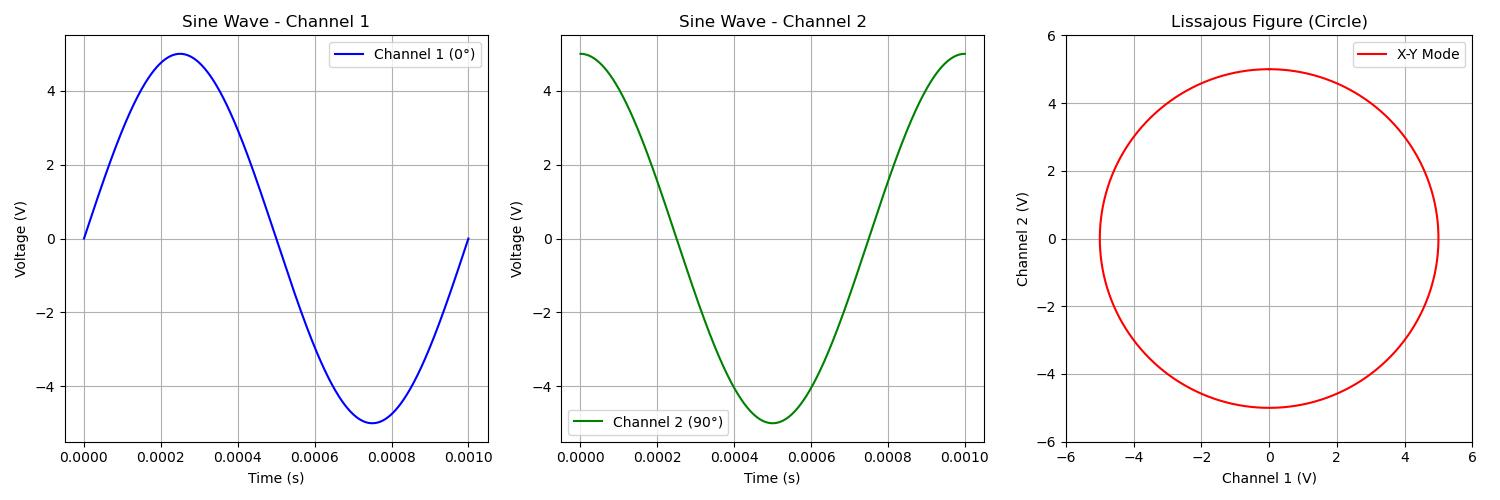
\includegraphics[width=\textwidth]{figs/2.jpg} % Replace "1.jpg" with your actual image filename
    \begin{minipage}[c]{0.48\textwidth}
        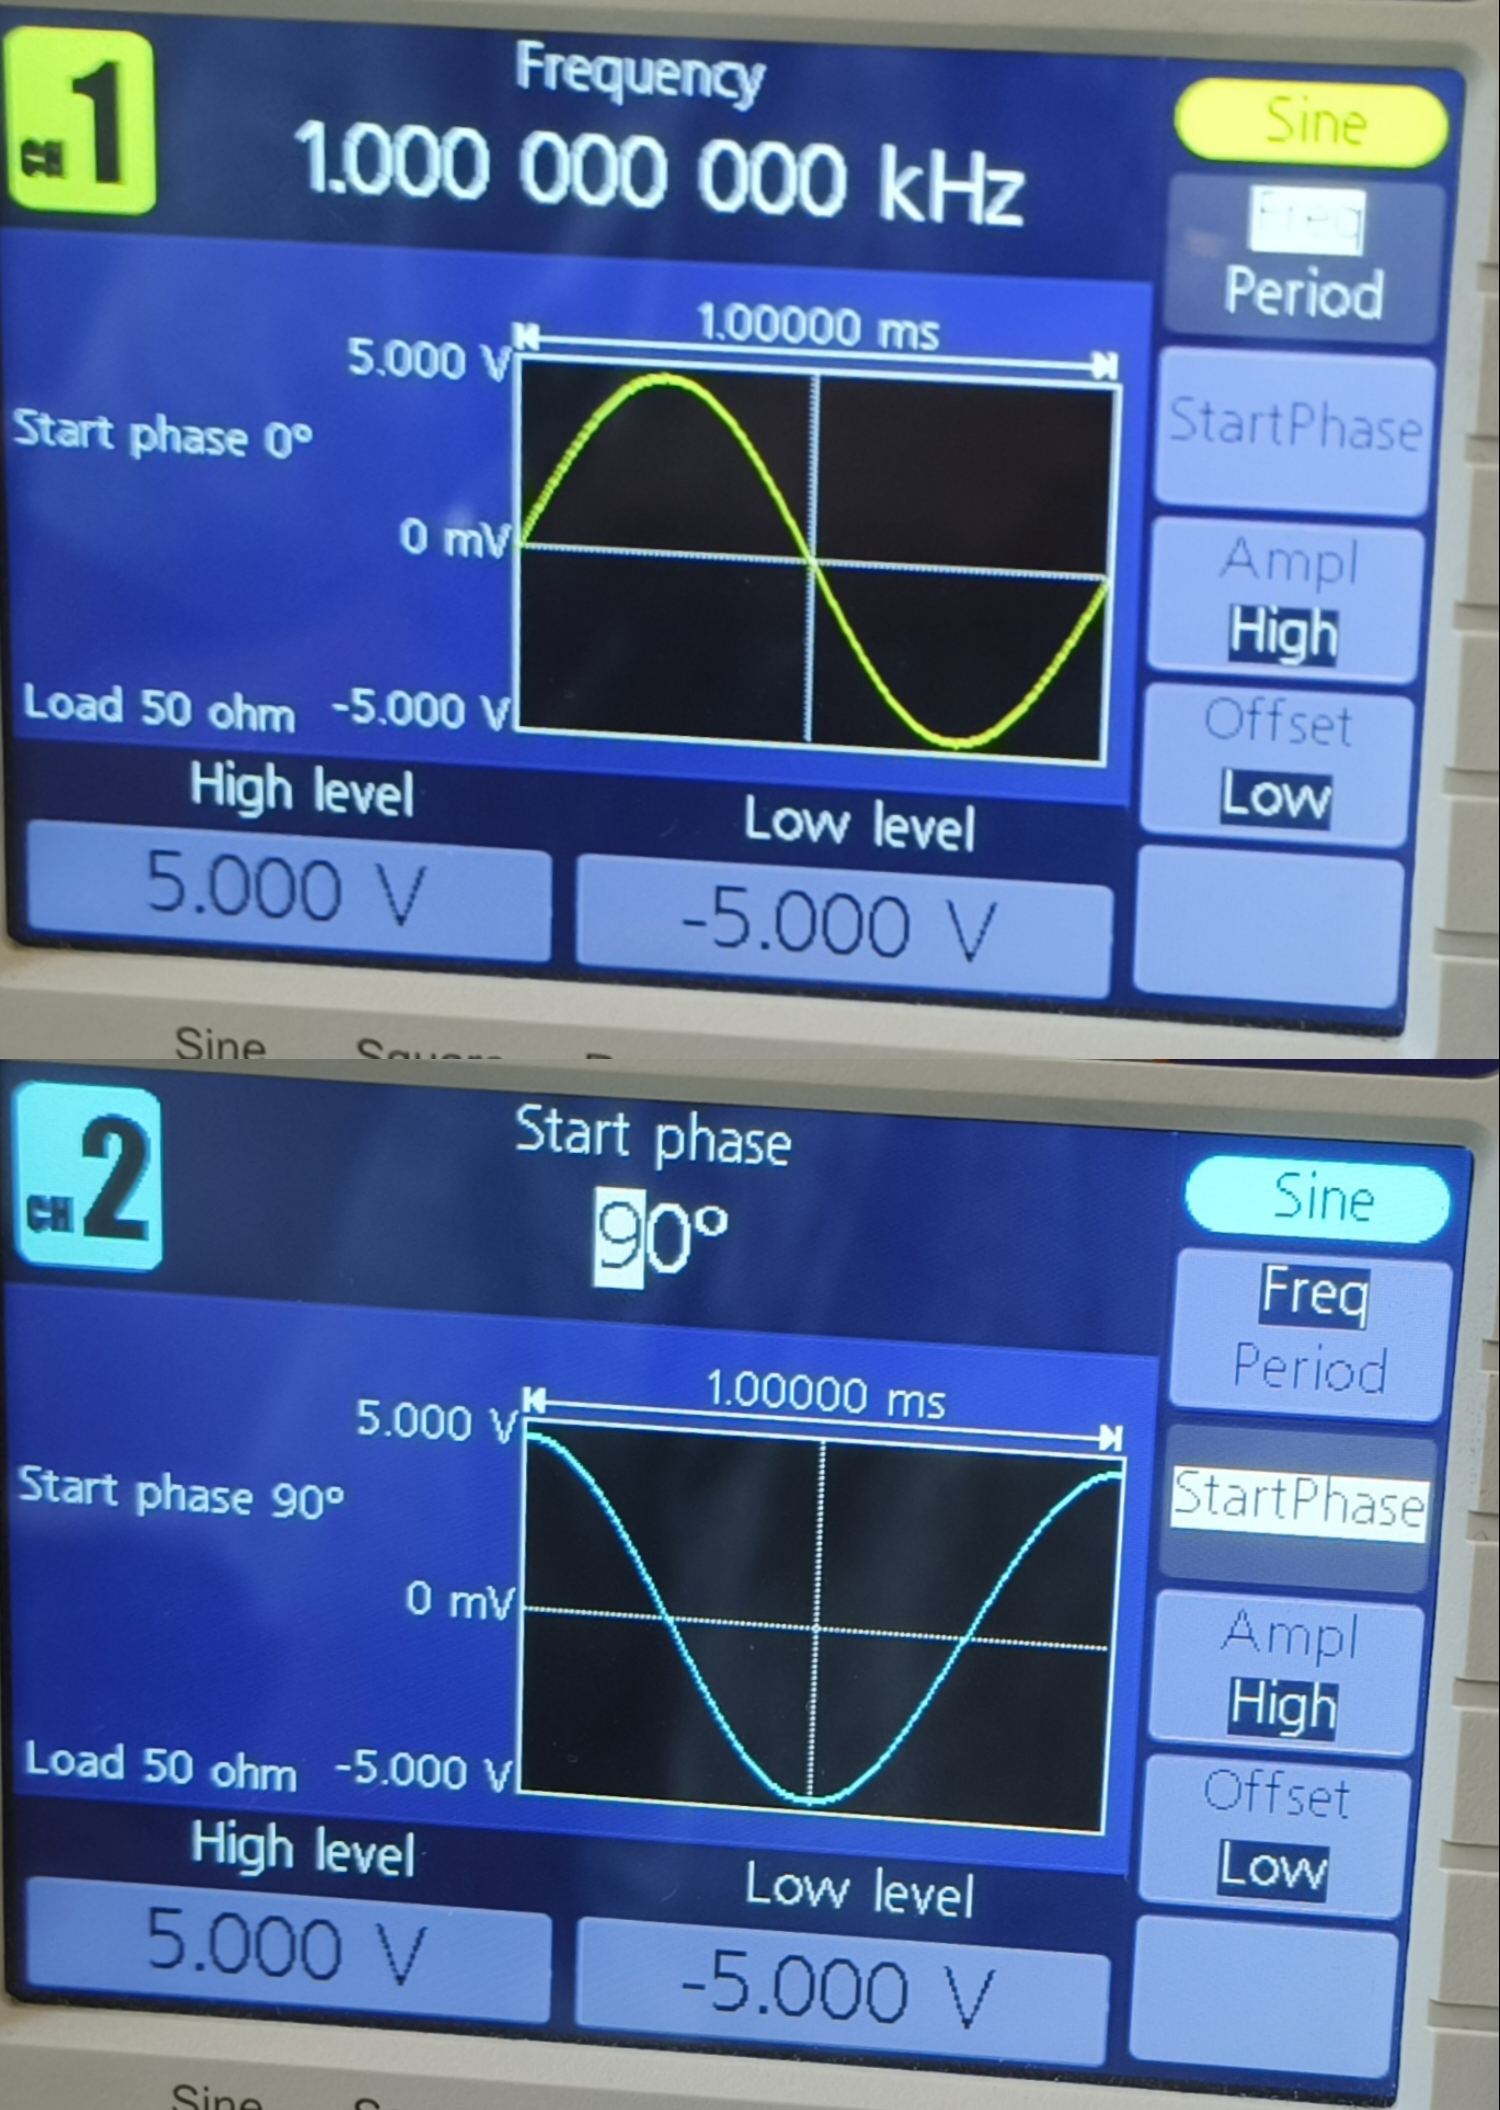
\includegraphics[width=\textwidth]{figs/2read.jpg} % Replace with the actual file name
        
    \end{minipage}
    \hfill
    \begin{minipage}[c]{0.48\textwidth}
        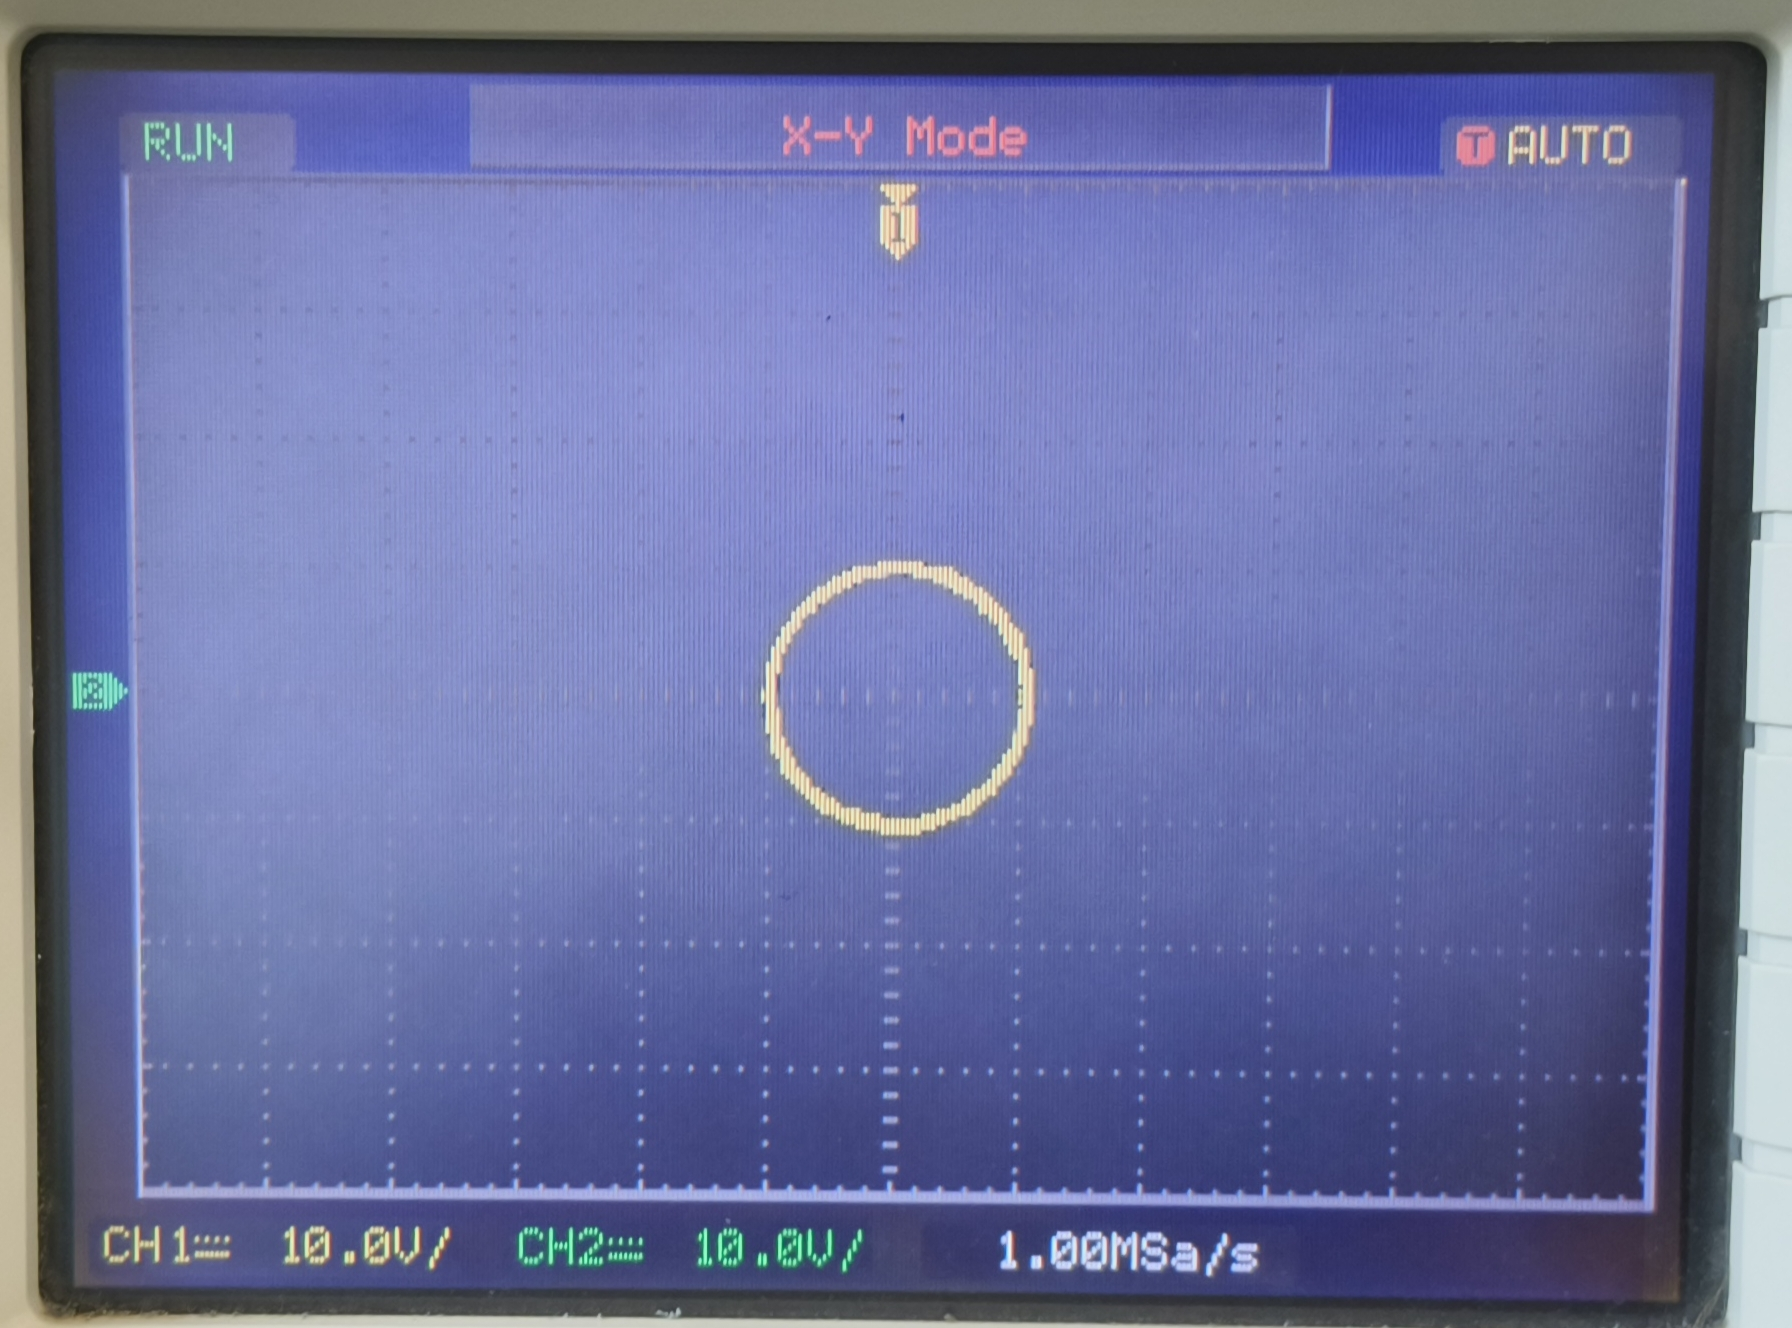
\includegraphics[width=\textwidth]{figs/2cro.jpg} % Replace with the actual file name
        
    \end{minipage}
    \caption{Graph 2}
    \label{fig:CRO-patterns}
\end{figure}
\subsubsection*{Conclusion}
The observed circular Lissajous figure confirms that:
\begin{itemize}
    \item The two sine waves have the same frequency (\(f_1 = f_2\)).
    \item The signals are \(90^\circ\) out of phase (\(\Delta \phi = \pi/2\)).
\end{itemize}
This analysis demonstrates the geometric relationship between the two signals and their phase difference.

\subsection{Three}
The two sine waves are represented as:
\[
V_1(t) = A_1 \sin(2 \pi f_1 t + \phi_1)
\]
\[
V_2(t) = A_2 \sin(2 \pi f_2 t + \phi_2)
\]

For the frequency ratio $f_1 : f_2 = 1 : 2$:
\begin{itemize}
    \item $f_1 = f$ (frequency of the first wave),
    \item $f_2 = 2f$ (frequency of the second wave).
\end{itemize}
Substituting these values:
\[
x(t) = A_1 \sin(2 \pi f t + \phi_1)
\]
\[
y(t) = A_2 \sin(4 \pi f t + \phi_2)
\]

\subsubsection*{Frequency Analysis}
The ratio $f_1 : f_2 = 1 : 2$ implies that:
\begin{itemize}
    \item The $x$-axis signal completes one oscillation in time $T_x = \frac{1}{f}$.
    \item The $y$-axis signal completes two oscillations in the same time $T_x$ (since $f_2 = 2f_1$).
\end{itemize}
This results in a closed figure with symmetry, forming a figure-eight pattern.

\subsubsection*{Parametric Representation}
To eliminate $t$, solve for $t$ from $x(t)$:
\[
x(t) = A_1 \sin(2 \pi f t + \phi_1)
\]
\[
\sin^{-1}\left(\frac{x}{A_1}\right) = 2 \pi f t + \phi_1
\]
\[
t = \frac{\sin^{-1}(x / A_1) - \phi_1}{2 \pi f}
\]

Substitute $t$ into $y(t)$:
\[
y = A_2 \sin\left[4 \pi f \cdot \frac{\sin^{-1}(x / A_1) - \phi_1}{2 \pi f} + \phi_2 \right]
\]
Simplify:
\[
y = A_2 \sin\left[2 \sin^{-1}(x / A_1) - 2 \phi_1 + \phi_2 \right]
\]

This parametric relationship generates the Lissajous figure.

\subsubsection*{Conclusion}
The Lissajous figure forms a closed curve because the frequency ratio is a simple integer ratio ($m : n = 1 : 2$). Specifically:
\begin{itemize}
    \item $x(t)$ completes one full cycle in time $T_x = \frac{1}{f_1}$.
    \item $y(t)$ completes two full cycles in the same time.
\end{itemize}
This results in the observed figure-eight pattern.


\subsubsection*{Figure of CRO Patterns}
\begin{figure}[H] % H forces the figure to be placed exactly here
    \centering
    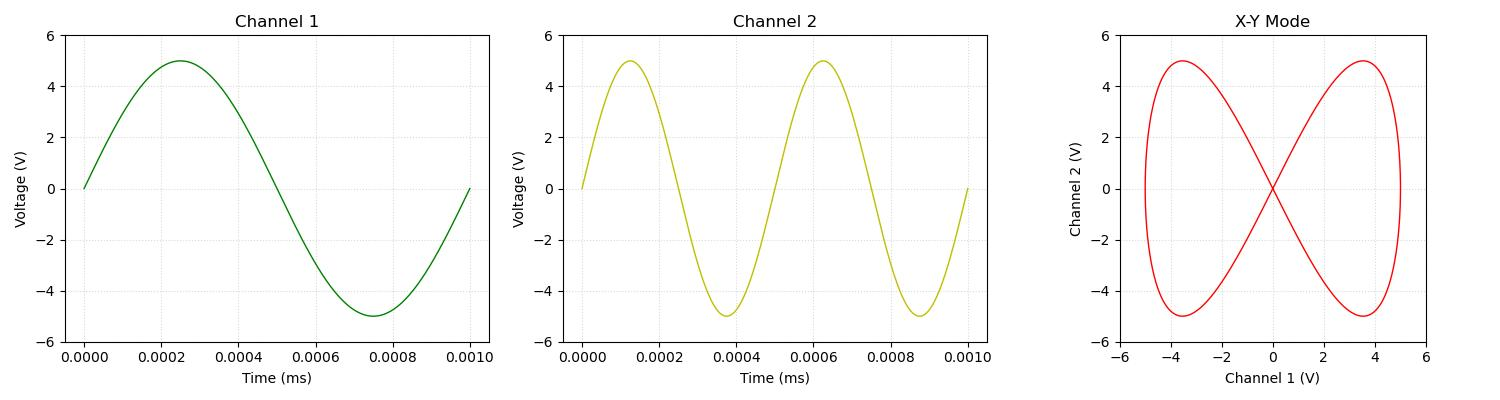
\includegraphics[width=\textwidth]{figs/3.jpg} % Replace "1.jpg" with your actual image filename
    \begin{minipage}[c]{0.48\textwidth}
        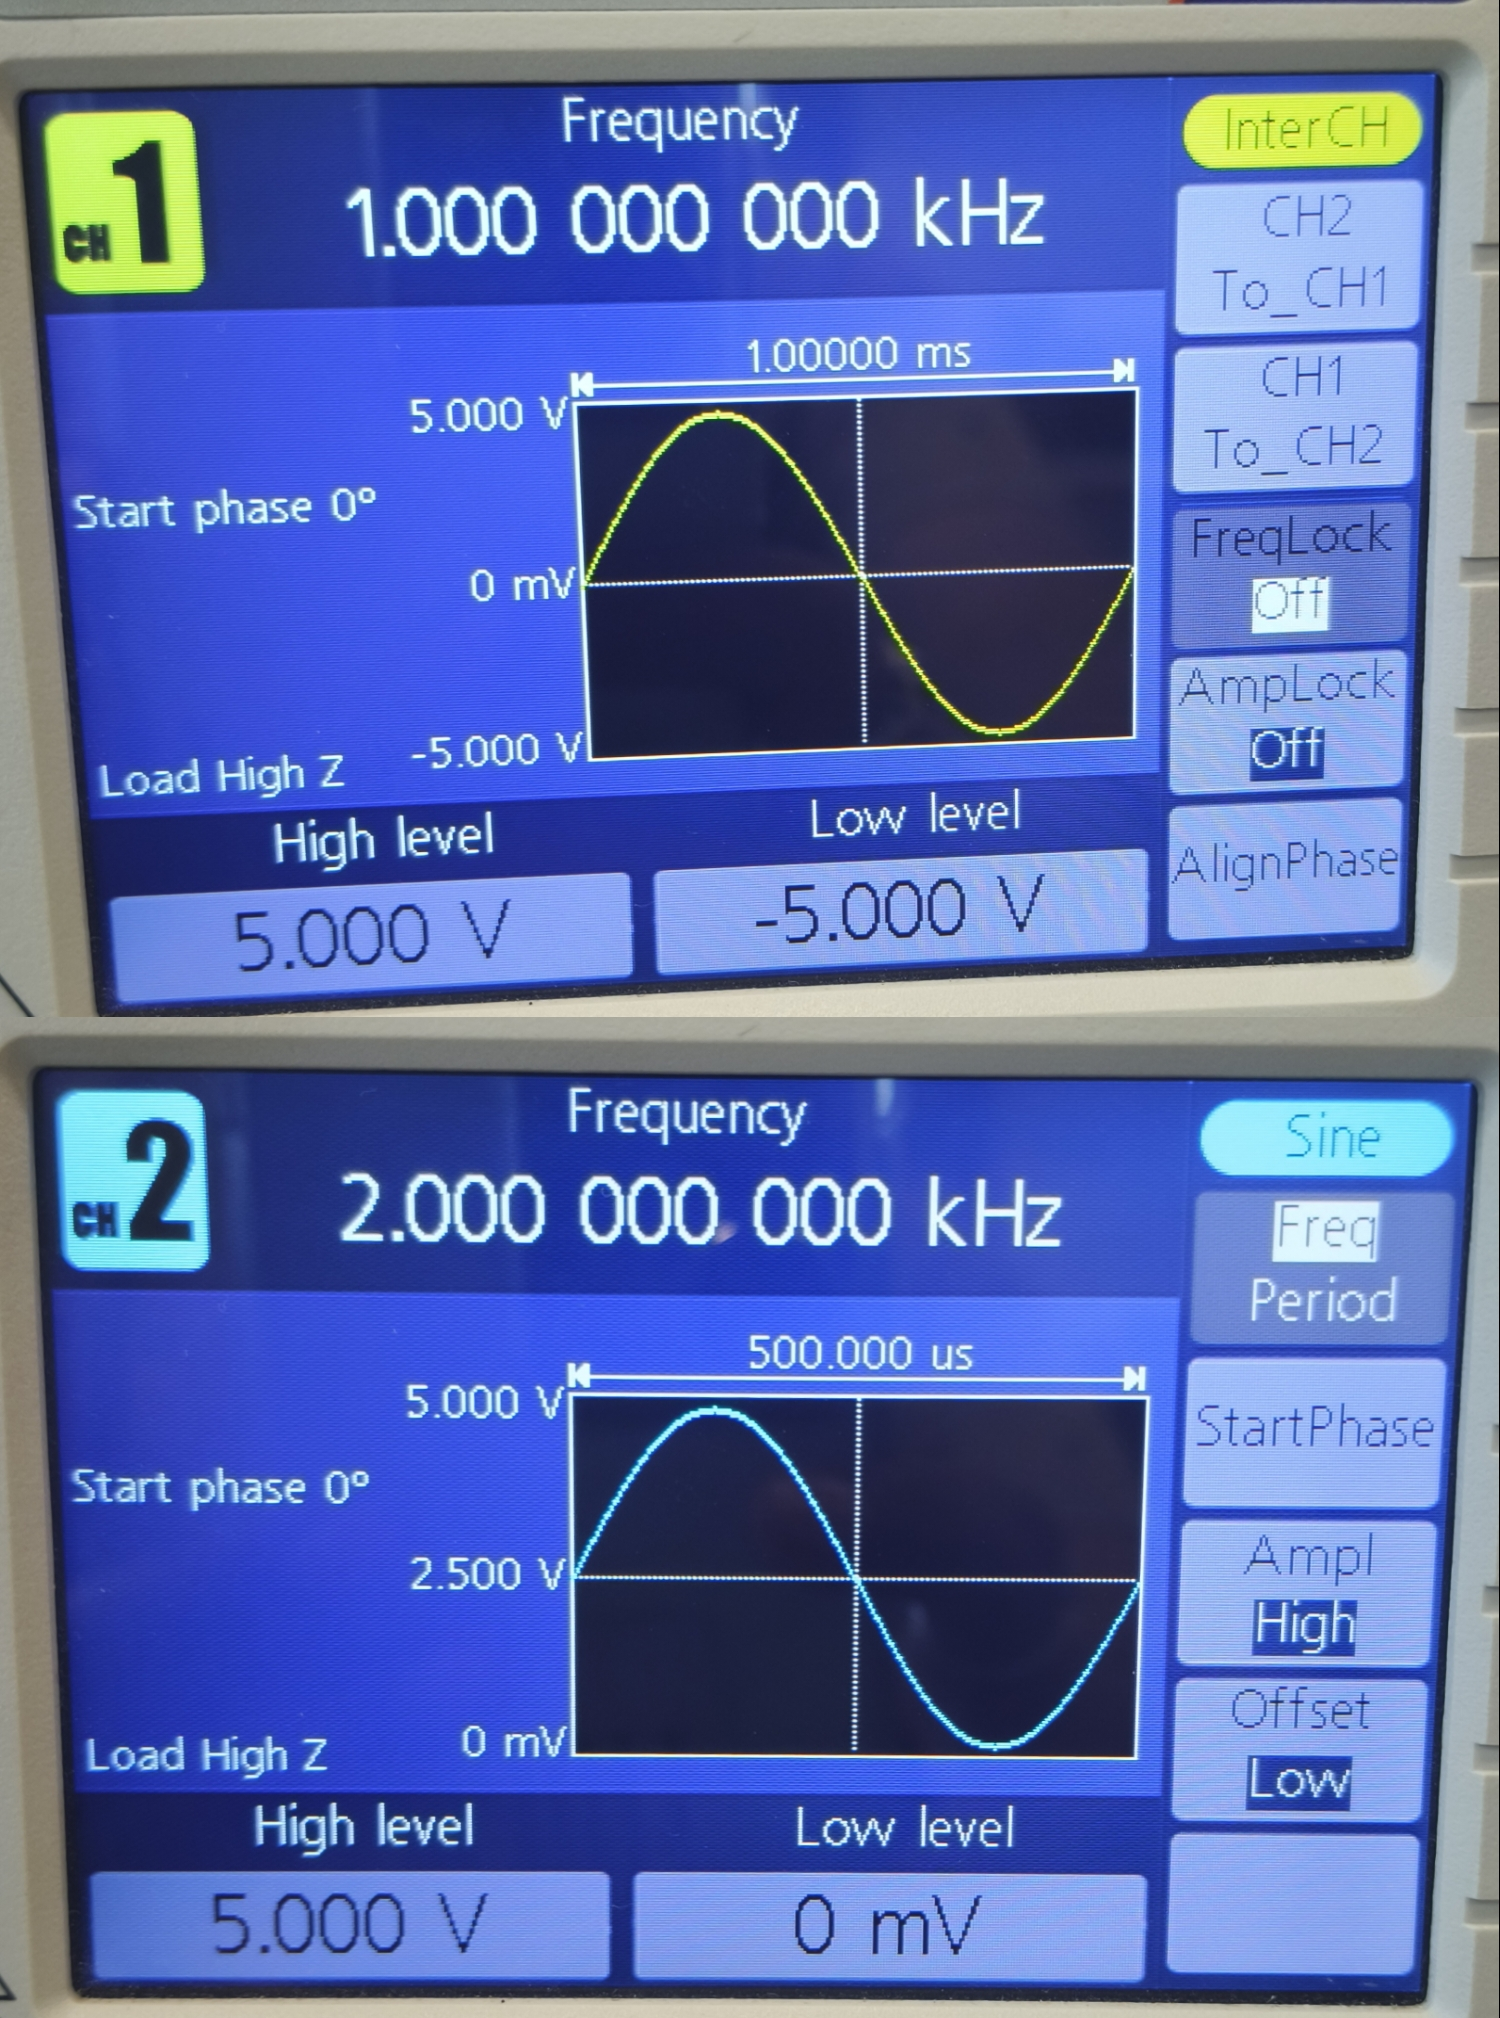
\includegraphics[width=\textwidth]{figs/3read.jpg} % Replace with the actual file name
        
    \end{minipage}
    \hfill
    \begin{minipage}[c]{0.48\textwidth}
        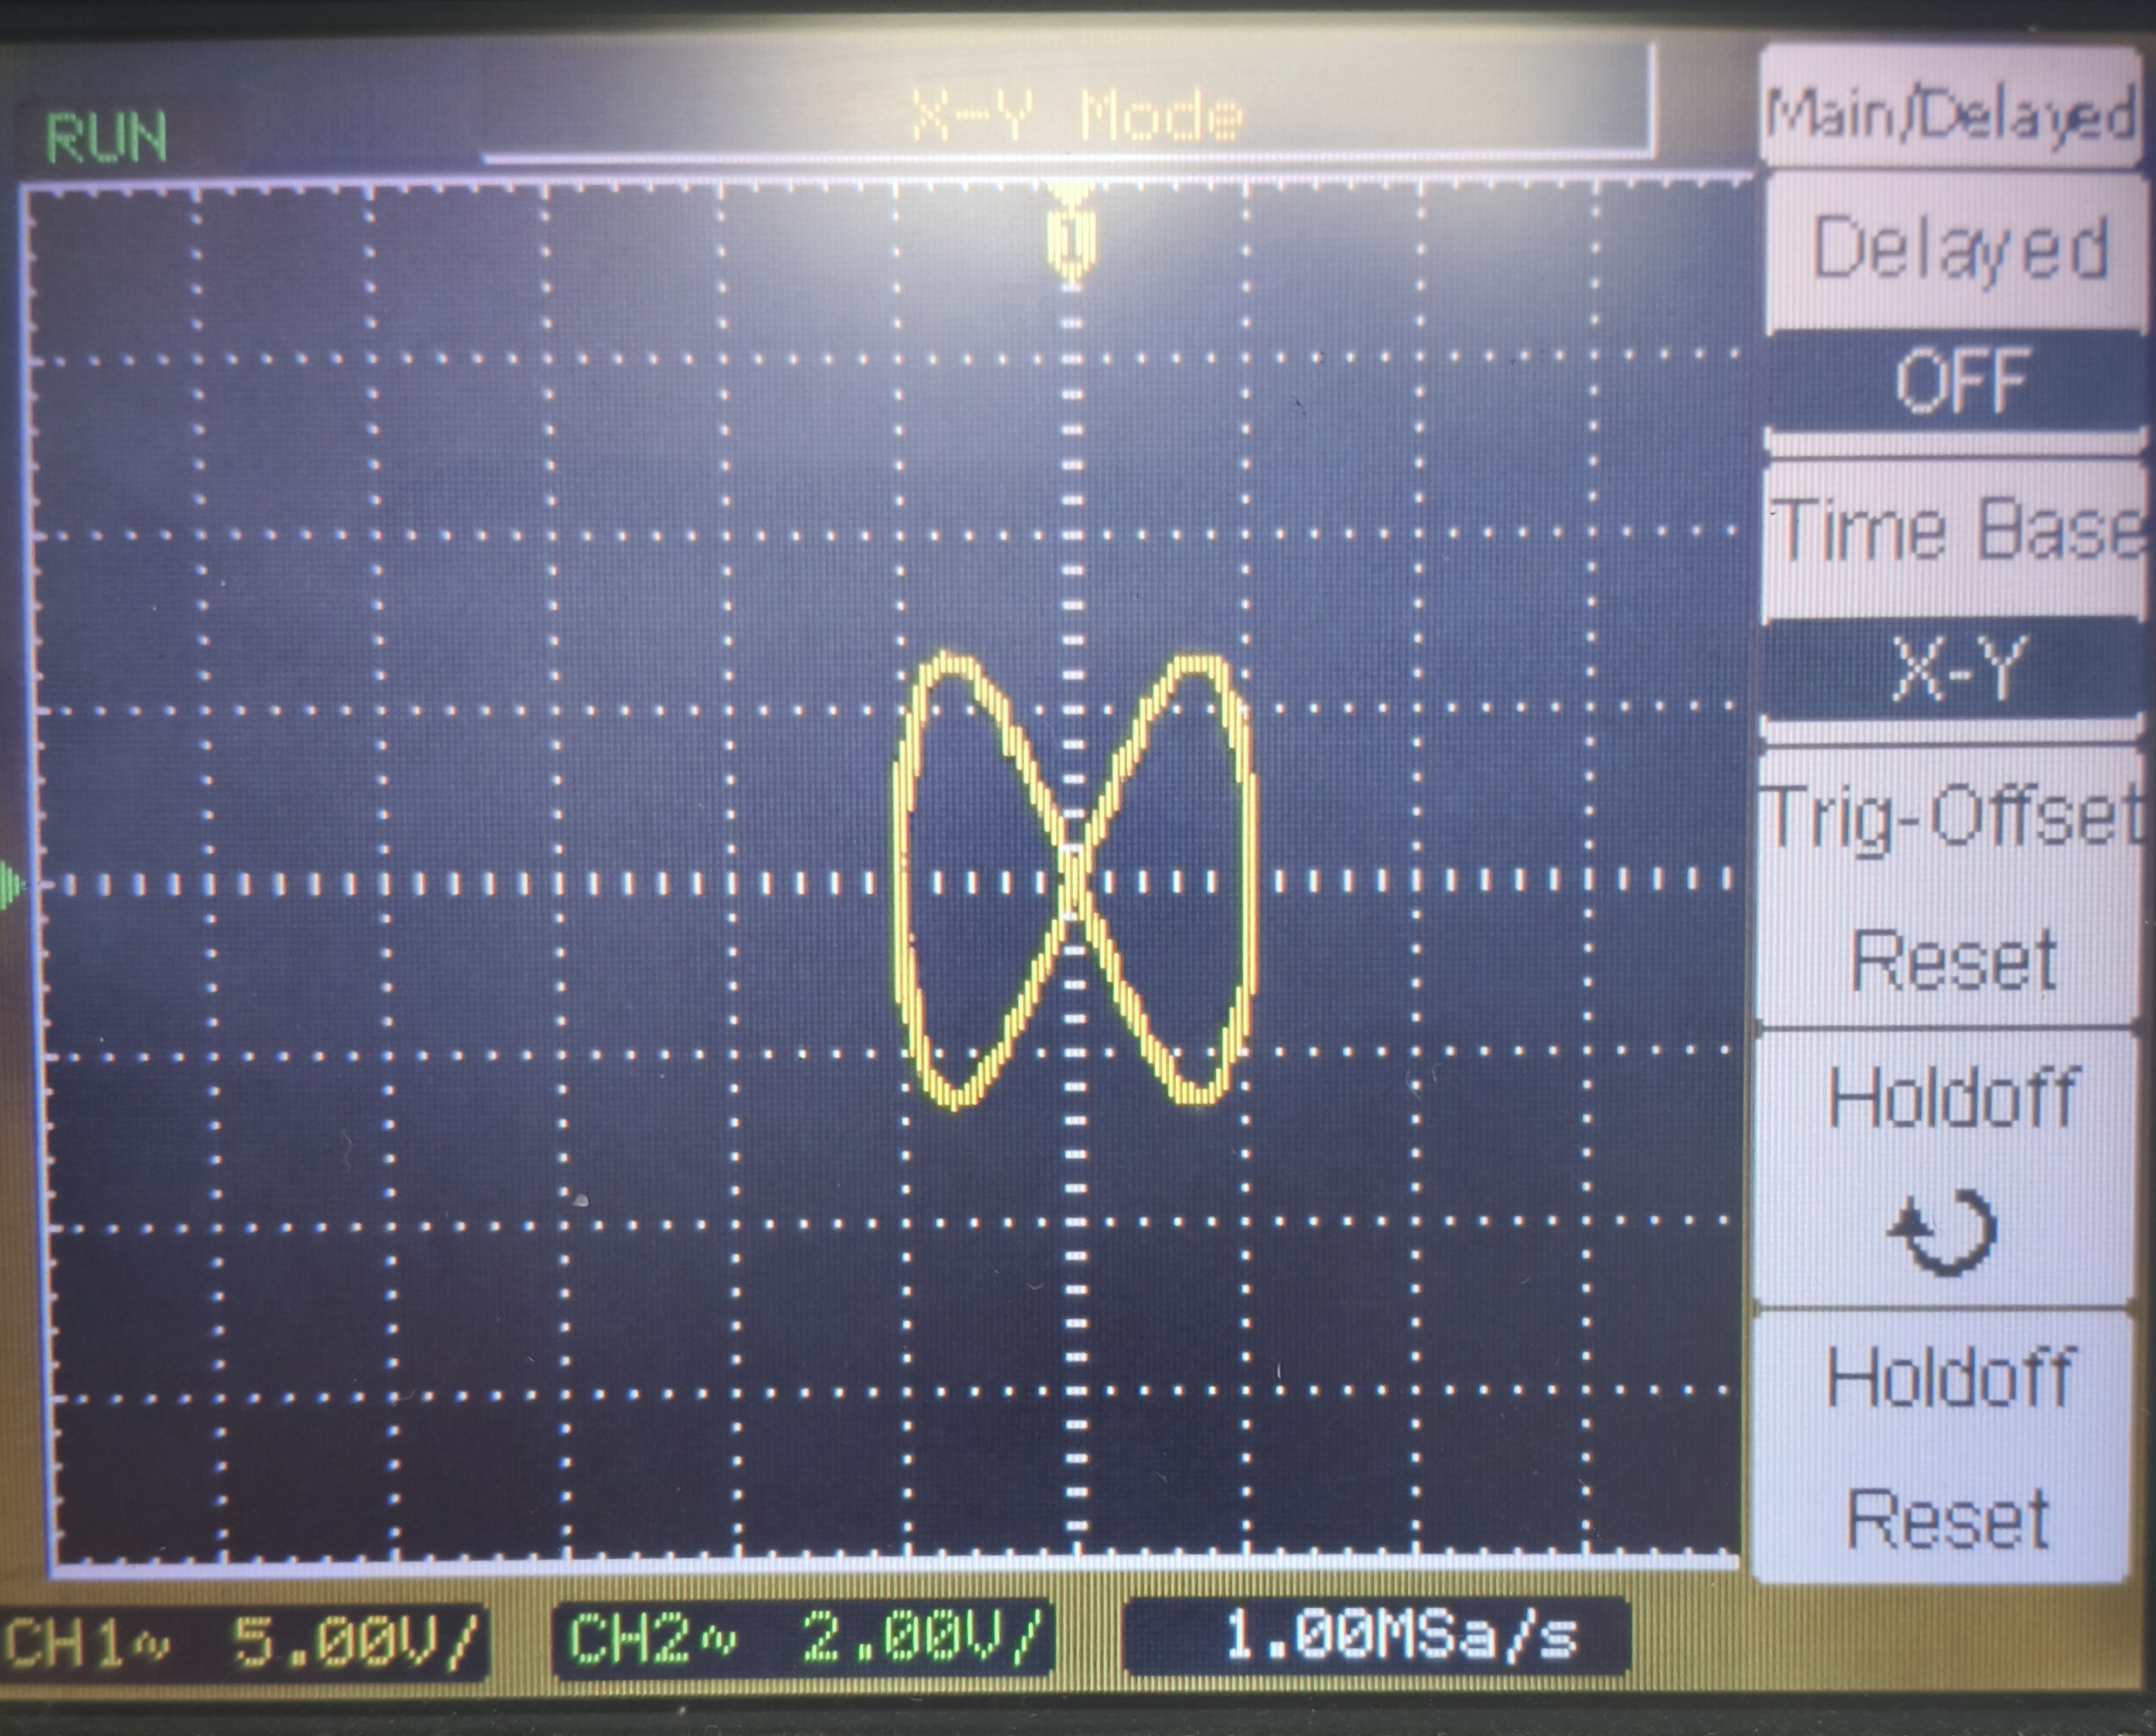
\includegraphics[width=\textwidth]{figs/3cro.jpg} % Replace with the actual file name
        
    \end{minipage}
    \caption{Graph 3}
    \label{fig:CRO-patterns}
\end{figure}
\subsection{Four}
The two sine waves are represented as:
\[
V_1(t) = A_1 \sin(2 \pi f_1 t + \phi_1)
\]
\[
V_2(t) = A_2 \sin(2 \pi f_2 t + \phi_2)
\]

\subsection*{Case 1: Same Frequency (\(f_1 = f_2 = f\))}
If the two signals have the same frequency, the resulting Lissajous figure depends on the phase difference (\( \Delta \phi = \phi_2 - \phi_1 \)).

\begin{itemize}
    \item \(\Delta \phi = 0\): Signals are in phase, and the figure is a straight line with a positive slope.
    \item \(\Delta \phi = \pi/2\): Signals are \(90^\circ\) out of phase, producing a circle.
    \item \(\Delta \phi = \pi/4\): Signals have a phase difference of \(45^\circ\), producing an ellipse with a specific orientation.
    \item Arbitrary \(\Delta \phi\): The figure is an ellipse.
\end{itemize}

\subsection*{Parametric Representation}
The parametric equations for the Lissajous figure are:
\[figs/
x(t) = A_1 \sin(2 \pi f t + \phi_1)
\]
\[
y(t) = A_2 \sin(2 \pi f t + \phi_2)
\]

For a phase difference of \(\Delta \phi = \pi/4\), the equations become:
\[
x(t) = A \sin(2 \pi f t)
\]
\[
y(t) = A \sin(2 \pi f t + \pi/4)
\]

\subsection*{Mathematical Interpretation for Ellipse Formation}
The key to the elliptical Lissajous figure lies in the phase difference between the two signals. When the phase difference is \( \Delta \phi = \pi/4 \), we can derive the following:

1. **Rewriting the Equation for \(y(t)\)**:
   Using the trigonometric identity for \( \sin(a + b) \), we get:
   \[
   y(t) = A \left( \sin(2 \pi f t) \cos\left(\frac{\pi}{4}\right) + \cos(2 \pi f t) \sin\left(\frac{\pi}{4}\right) \right)
   \]
   Simplifying with \( \cos\left(\frac{\pi}{4}\right) = \sin\left(\frac{\pi}{4}\right) = \frac{\sqrt{2}}{2} \), this becomes:
   \[
   y(t) = A \frac{\sqrt{2}}{2} \left( \sin(2 \pi f t) + \cos(2 \pi f t) \right)
   \]

2. **Expressing \(y(t)\) in Terms of \(x(t)\)**:
   Since \( x(t) = A \sin(2 \pi f t) \), we can substitute into the equation for \(y(t)\):
   \[
   y(t) = \frac{\sqrt{2}}{2} \left( x(t) + A \cos(2 \pi f t) \right)
   \]
   This results in an elliptical curve on the X-Y plane with equal axes.

3. **Geometric Interpretation**:
   The phase difference causes the two sine waves to be offset, leading to an elliptical path. The equation describes an ellipse with equal axes because the amplitudes are the same. The general form of the ellipse is:
   \[
   \left(\frac{x}{A}\right)^2 + \left(\frac{y}{A}\right)^2 = 1
   \]
   The ellipse is rotated by \( \pi/4 \), as indicated by the phase shift between the two sine waves.

\subsection*{Observed Lissajous Pattern}
From the provided CRO plots:
\begin{itemize}
    \item The sine wave in \textbf{Channel 1} is:
    \[
    V_1(t) = A \sin(2 \pi f t)
    \]
    \item The sine wave in \textbf{Channel 2} is:
    \[
    V_2(t) = A \sin(2 \pi f t + \pi/4)
    \]
    \item The Lissajous figure in X-Y mode forms an ellipse, confirming the phase difference of \(45^\circ\) (\(\pi/4\)).
\end{itemize}

\subsubsection*{Figure of CRO Patterns}
\begin{figure}[H] % H forces the figure to be placed exactly here
    \centering
    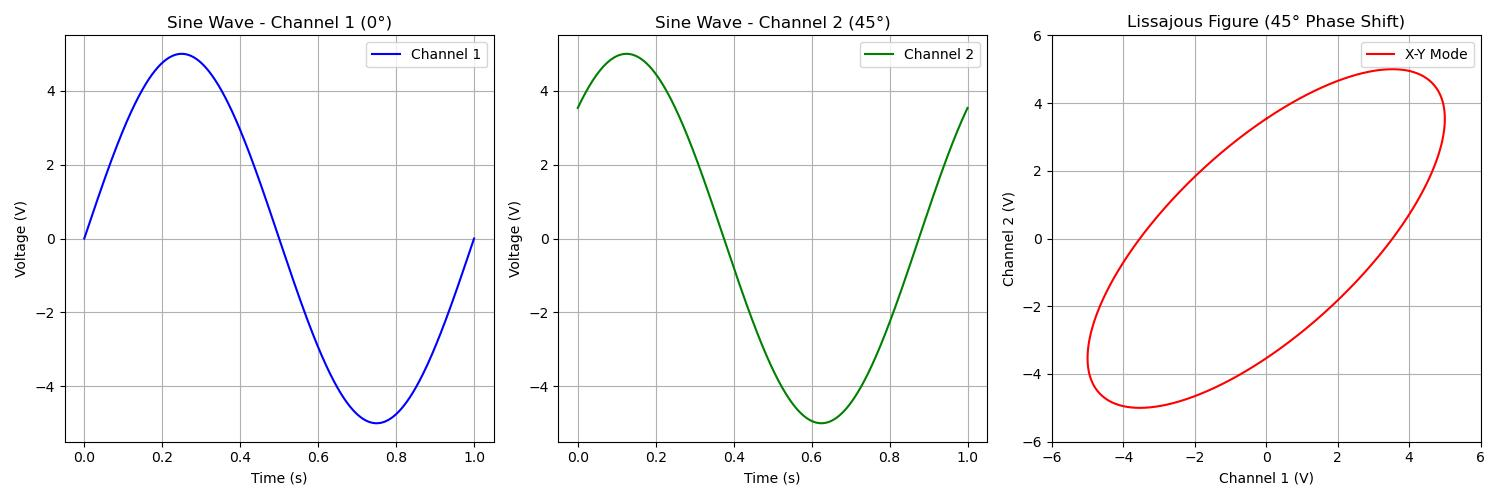
\includegraphics[width=\textwidth]{figs/4.jpg} % Replace "1.jpg" with your actual image filename
    \begin{minipage}[c]{0.48\textwidth}
        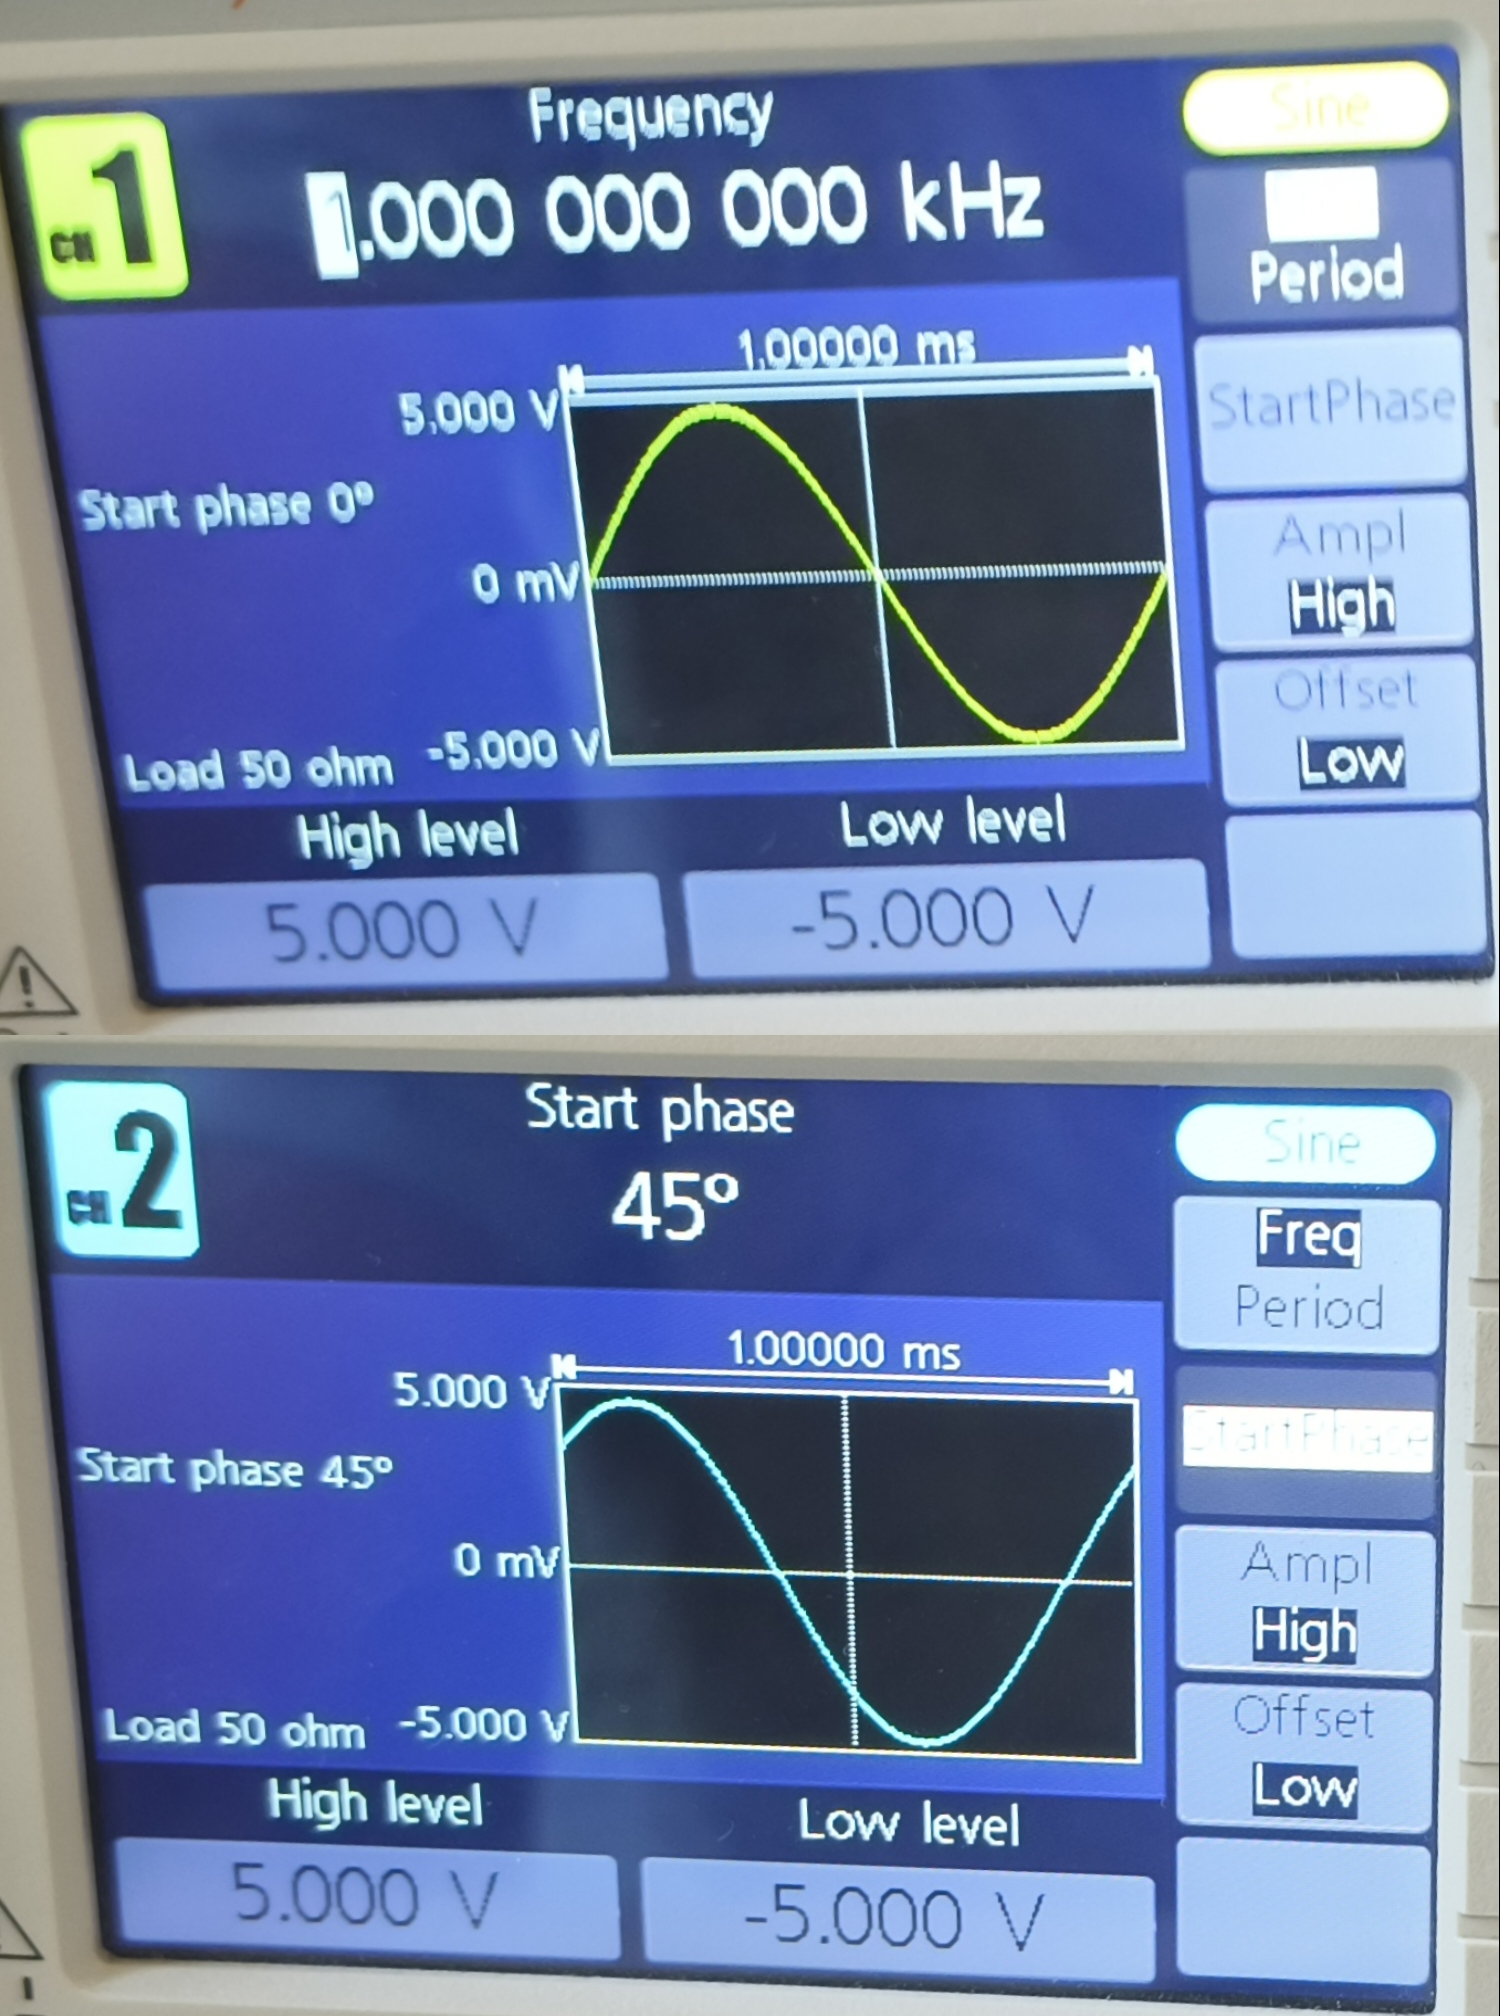
\includegraphics[width=\textwidth]{figs/4read.jpg} % Replace with the actual file name
        
    \end{minipage}
    \hfill
    \begin{minipage}[c]{0.48\textwidth}
        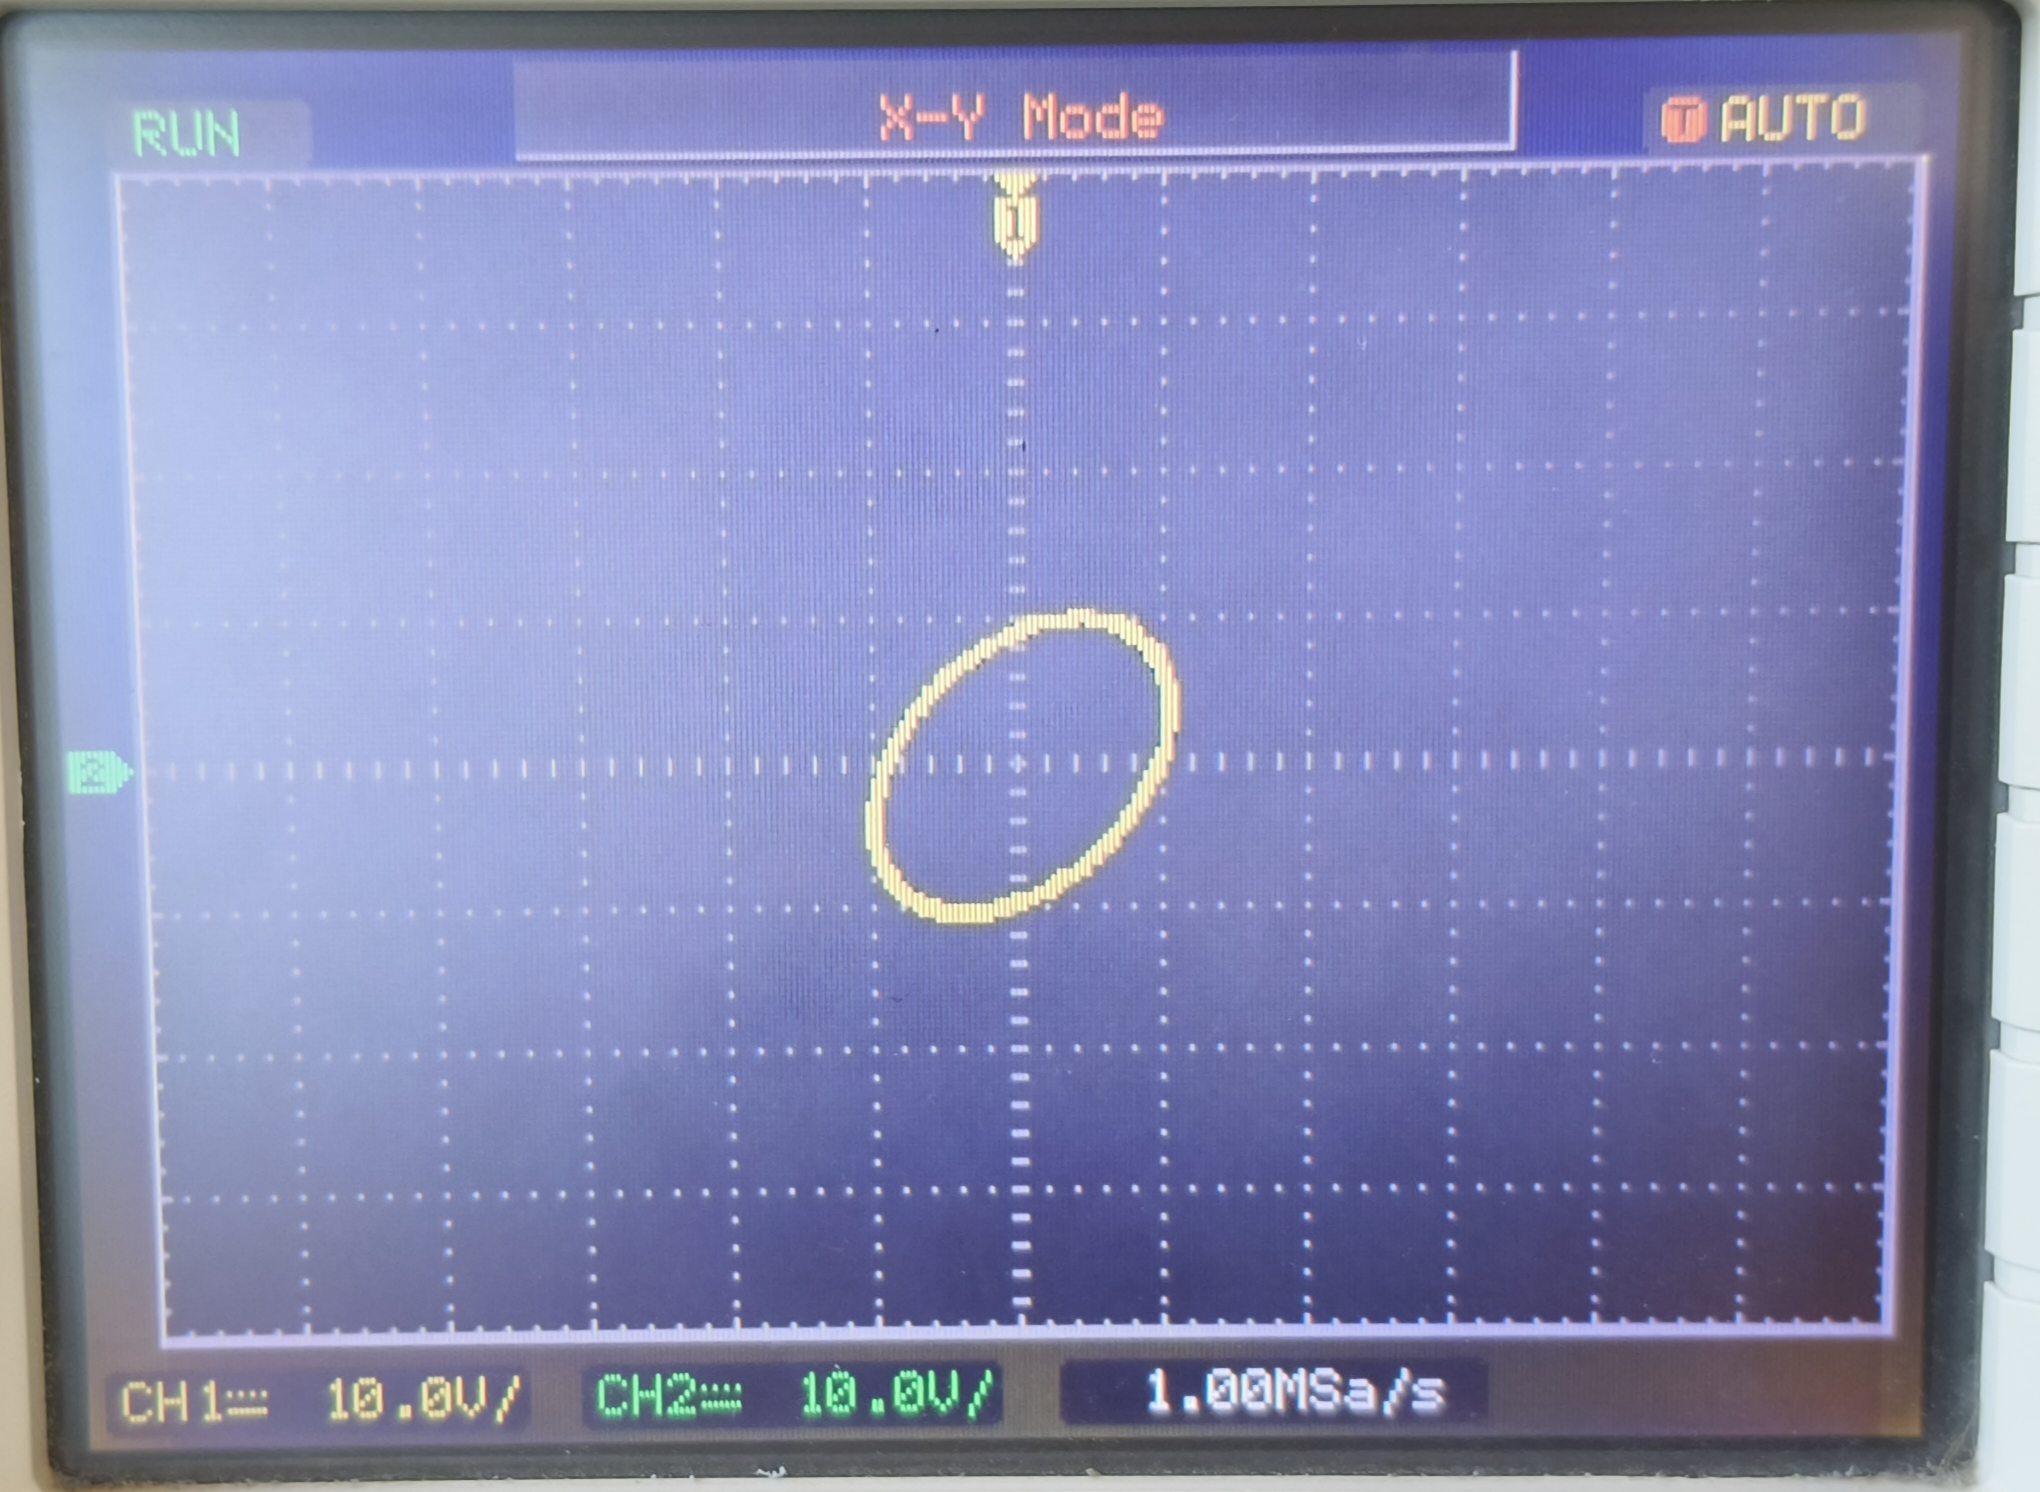
\includegraphics[width=\textwidth]{figs/4cro.jpg} % Replace with the actual file name
        
    \end{minipage}
    \caption{Graph 4}
    \label{fig:CRO-patterns}
\end{figure}


\subsection*{Step-by-Step Justification}
\begin{enumerate}
    \item \textbf{Equal Frequencies:} Both sine waves have the same frequency \(f\), ensuring a consistent Lissajous figure.
    \item \textbf{Phase Difference:} The phase difference of \(\Delta \phi = \pi/4\) leads to an elliptical pattern due to the sine wave offsets.
    \item \textbf{Amplitude:} Both waves have the same amplitude \(A\), resulting in a symmetric ellipse.
    \item \textbf{Observation:} On the CRO in X-Y mode:
    \begin{itemize}
        \item Channel 1 displays \(V_1(t) = A \sin(2 \pi f t)\).
        \item Channel 2 displays \(V_2(t) = A \sin(2 \pi f t + \pi/4)\).
        \item The resulting ellipse confirms the phase relationship and equal frequencies.
    \end{itemize}
\end{enumerate}

\subsection*{Conclusion}
The observed elliptical Lissajous figure confirms that:
\begin{itemize}
    \item The two sine waves have the same frequency (\(f_1 = f_2\)).
    \item The signals have a phase difference of \(45^\circ\) (\(\pi/4\)).
\end{itemize}
This analysis demonstrates the geometric relationship between the two signals and their phase difference as seen on the CRO.
\subsection{Five}
The two sine waves are represented as:
\[
V_1(t) = A_1 \sin(2 \pi f_1 t + \phi_1)
\]
\[
V_2(t) = A_2 \sin(2 \pi f_2 t + \phi_2)
\]

For the frequency ratio $f_1 : f_2 = 1 : 2$:
\begin{itemize}
    \item $f_1 = f$ (frequency of the first wave),
    \item $f_2 = 2f$ (frequency of the second wave).
\end{itemize}
Substituting these values:
\[
x(t) = A_1 \sin(2 \pi f t + \phi_1)
\]
\[
y(t) = A_2 \sin(4 \pi f t + \phi_2)
\]

The phase shift in the second channel is introduced as:
\[
\phi_2 = \frac{\pi}{4}
\]

Thus, the second wave becomes:
\[
y(t) = A_2 \sin(4 \pi f t + \frac{\pi}{4})
\]

\subsection*{Frequency Analysis}
The ratio $f_1 : f_2 = 1 : 2$ implies that:
\begin{itemize}
    \item The $x$-axis signal completes one oscillation in time $T_x = \frac{1}{f}$.
    \item The $y$-axis signal completes two oscillations in the same time $T_x$ (since $f_2 = 2f_1$).
\end{itemize}
This results in a closed figure with symmetry, but the additional phase shift will distort the shape of the figure.

\subsection*{Parametric Representation}
To eliminate $t$, solve for $t$ from $x(t)$:
\[
x(t) = A_1 \sin(2 \pi f t + \phi_1)
\]
\[
\sin^{-1}\left(\frac{x}{A_1}\right) = 2 \pi f t + \phi_1
\]
\[
t = \frac{\sin^{-1}(x / A_1) - \phi_1}{2 \pi f}
\]

Substitute $t$ into $y(t)$:
\[
y = A_2 \sin\left[4 \pi f \cdot \frac{\sin^{-1}(x / A_1) - \phi_1}{2 \pi f} + \frac{\pi}{4}\right]
\]
Simplify:
\[
y = A_2 \sin\left[2 \sin^{-1}(x / A_1) - 2 \phi_1 + \frac{\pi}{4}\right]
\]

This parametric relationship generates the modified Lissajous figure with the phase shift.

\subsection*{Pattern Closure}
The Lissajous figure forms a closed curve because the frequency ratio is a simple integer ratio ($m : n = 1 : 2$). Specifically:
\begin{itemize}
    \item $x(t)$ completes one full cycle in time $T_x = \frac{1}{f_1}$.
    \item $y(t)$ completes two full cycles in the same time.
\end{itemize}
However, the additional phase shift of \( \frac{\pi}{4} \) in the second channel introduces a rotation of the figure, changing the symmetry and shape compared to the standard figure-eight pattern.

\subsection*{Conclusion}
The modified Lissajous figure is a direct consequence of the $1 : 2$ frequency ratio and the additional phase shift of \( \frac{\pi}{4} \) in the second wave. This phase shift results in a rotated figure-eight pattern, altering the symmetry and creating a new characteristic shape.

\subsubsection*{Figure of CRO Patterns}
\begin{figure}[H] % H forces the figure to be placed exactly here
    \centering
    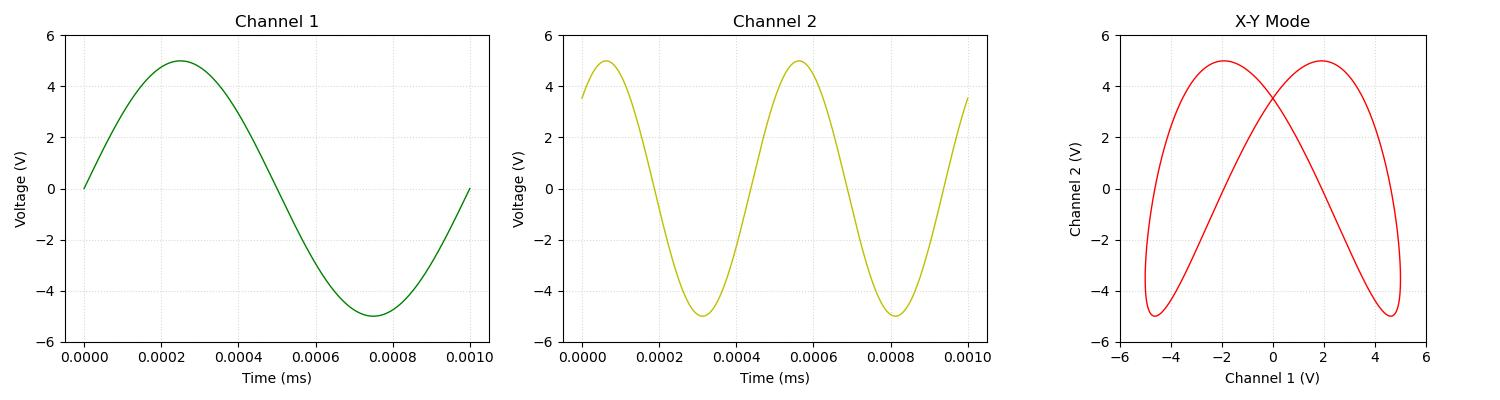
\includegraphics[width=\textwidth]{figs/5.jpg} % Replace "1.jpg" with your actual image filename
    \begin{minipage}[c]{0.48\textwidth}
        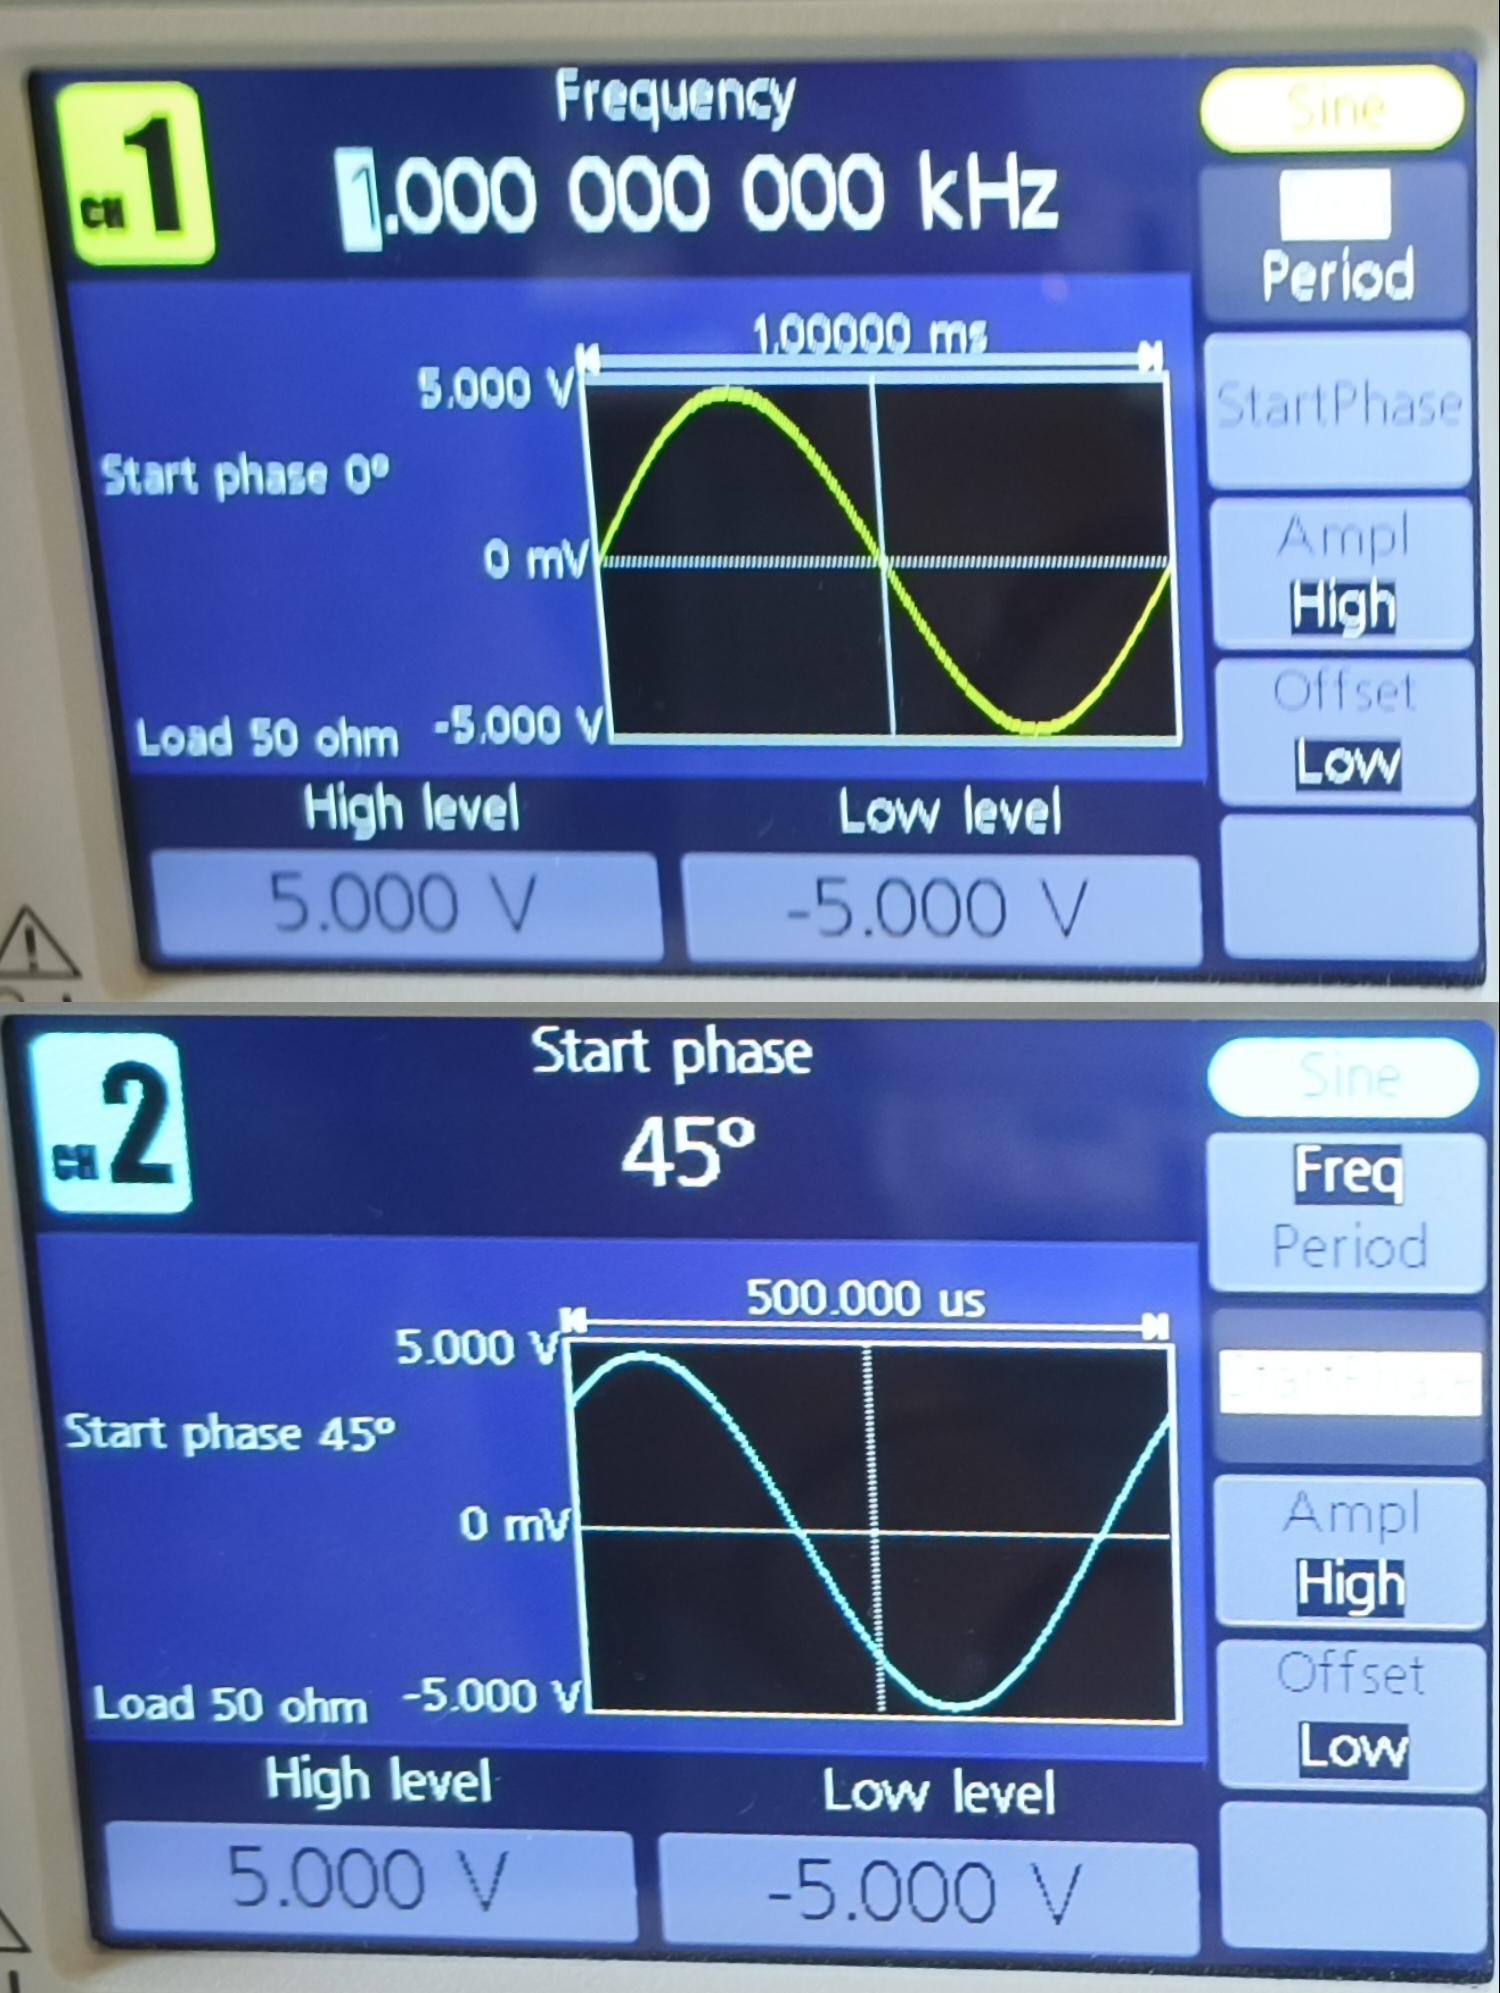
\includegraphics[width=\textwidth]{figs/5read.jpg} % Replace with the actual file name
        
    \end{minipage}
    \hfill
    \begin{minipage}[c]{0.48\textwidth}
        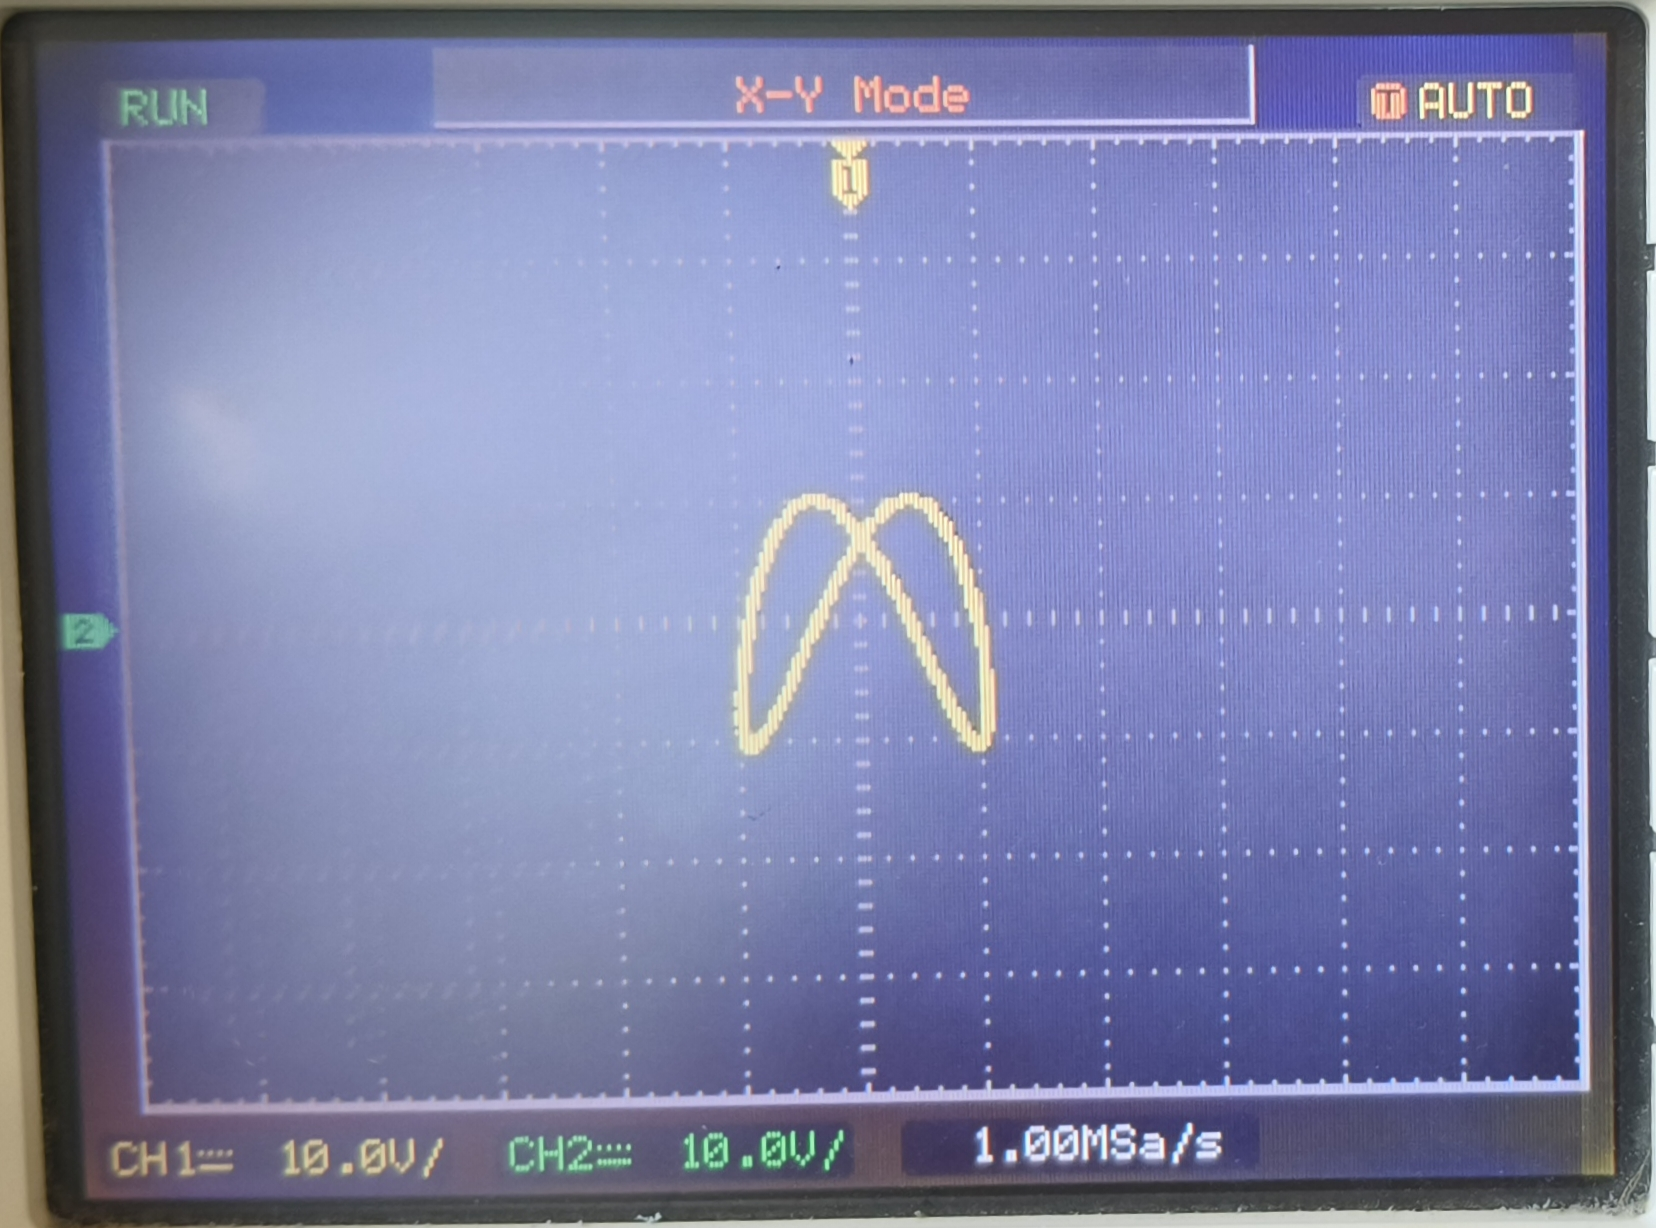
\includegraphics[width=\textwidth]{figs/5cro.jpg} % Replace with the actual file name
        
    \end{minipage}
    \caption{Graph 5}
    \label{fig:CRO-patterns}
\end{figure}
\subsection{Six}
The two waves are represented as:
\[
V_1(t) = A_1 \sin(2 \pi f t + \phi_1)
\]
\[
V_2(t) = A_2 \cdot \text{sgn}\left( \sin(2 \pi f t + \phi_2) \right)
\]

For the frequency and phase matching:
\begin{itemize}
    \item $f_1 = f_2 = f$ (same frequency),
    \item $\phi_1 = \phi_2 = \phi$ (same phase).
\end{itemize}

Substituting these values:
\[
x(t) = A_1 \sin(2 \pi f t + \phi)
\]
\[
y(t) = A_2 \cdot \text{sgn}\left( \sin(2 \pi f t + \phi) \right)
\]

Where \( \text{sgn}(x) \) is the sign function, defined as:
\[
\text{sgn}(x) = \begin{cases} 
1 & \text{if } x \geq 0 \\
-1 & \text{if } x < 0 
\end{cases}
\]

\subsection*{Frequency and Amplitude Analysis}
Since both waves have the same frequency and phase:
\begin{itemize}
    \item The sine wave completes one oscillation in time $T_x = \frac{1}{f}$.
    \item The square wave also completes one cycle in the same time, alternating between \( A_2 \) and \( -A_2 \).
\end{itemize}

The maximum value of \( y(t) \) in the square wave is determined directly by \( A_2 \). Thus:
\[
y_{\text{max}} = A_2
\]

The resulting pattern will exhibit sharp transitions due to the square wave but will retain the overall oscillatory behavior driven by the sine wave.

\subsection*{Parametric Representation}
To eliminate \( t \), solve for \( t \) from \( x(t) \):
\[
x(t) = A_1 \sin(2 \pi f t + \phi)
\]
\[
\sin^{-1}\left(\frac{x}{A_1}\right) = 2 \pi f t + \phi
\]
\[
t = \frac{\sin^{-1}(x / A_1) - \phi}{2 \pi f}
\]

Substitute \( t \) into \( y(t) \):
\[
y = A_2 \cdot \text{sgn}\left( \sin\left(2 \pi f \cdot \frac{\sin^{-1}(x / A_1) - \phi}{2 \pi f} + \phi \right) \right)
\]
Simplify:
\[
y = A_2 \cdot \text{sgn}\left( \sin\left( \sin^{-1}(x / A_1) \right) \right)
\]
Since \( \sin(\sin^{-1}(x / A_1)) = x / A_1 \), this becomes:
\[
y = A_2 \cdot \text{sgn}\left( x / A_1 \right)
\]
So:
\[
y = A_2 \cdot \begin{cases} 
1 & \text{if } x \geq 0 \\
-1 & \text{if } x < 0
\end{cases}
\]

\subsection*{Pattern Formation}
The Lissajous-like pattern in this case is characterized by:
\begin{itemize}
    \item A smooth oscillation in the \( x \)-axis (sine wave),
    \item A square, alternating oscillation in the \( y \)-axis.
\end{itemize}
Due to the sharp transitions in the square wave, the figure exhibits abrupt changes in the \( y \)-direction, creating a stepped pattern along the sine wave's trajectory.

\subsection*{Conclusion}
The pattern formed by the sine and square waves with the same frequency and phase results in:
\begin{itemize}
    \item A smooth oscillation in the \( x \)-axis with amplitude \( A_1 \),
    \item A discrete oscillation in the \( y \)-axis between \( A_2 \) and \( -A_2 \).
\end{itemize}
The maximum value of \( y(t) \) in this pattern is directly determined by the amplitude \( A_2 \). The resultant graph alternates between \( y = A_2 \) and \( y = -A_2 \) while tracing the sine wave's smooth horizontal path.
\subsubsection*{Figure of CRO Patterns}
\begin{figure}[H] % H forces the figure to be placed exactly here
    \centering
    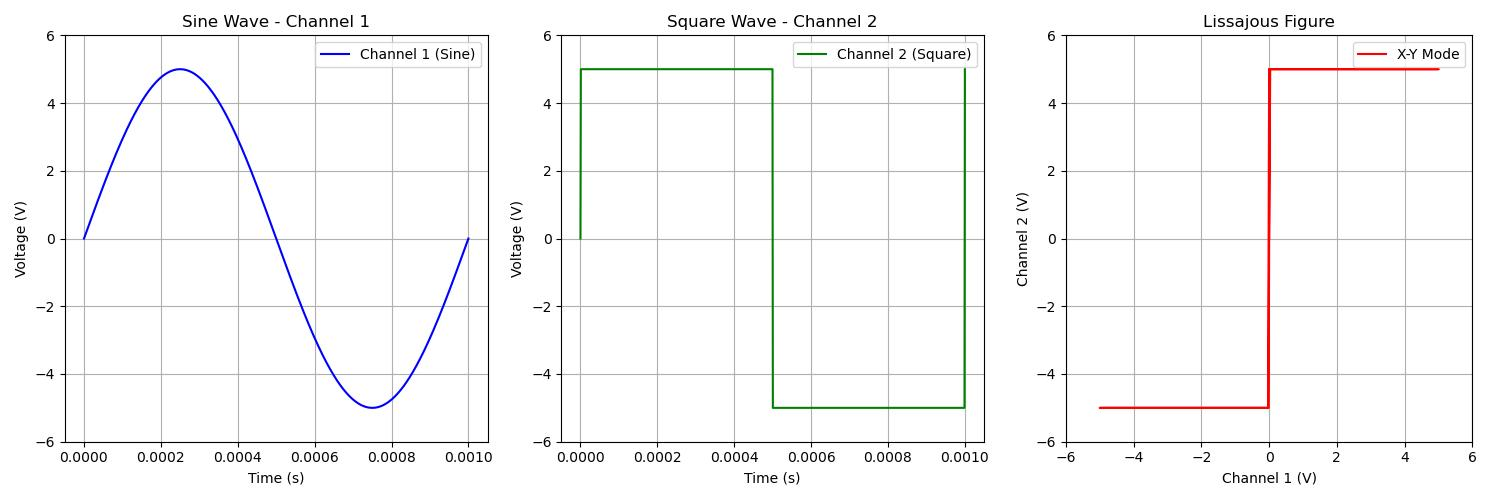
\includegraphics[width=\textwidth]{figs/6.jpg} % Replace "1.jpg" with your actual image filename
    \begin{minipage}[c]{0.48\textwidth}
        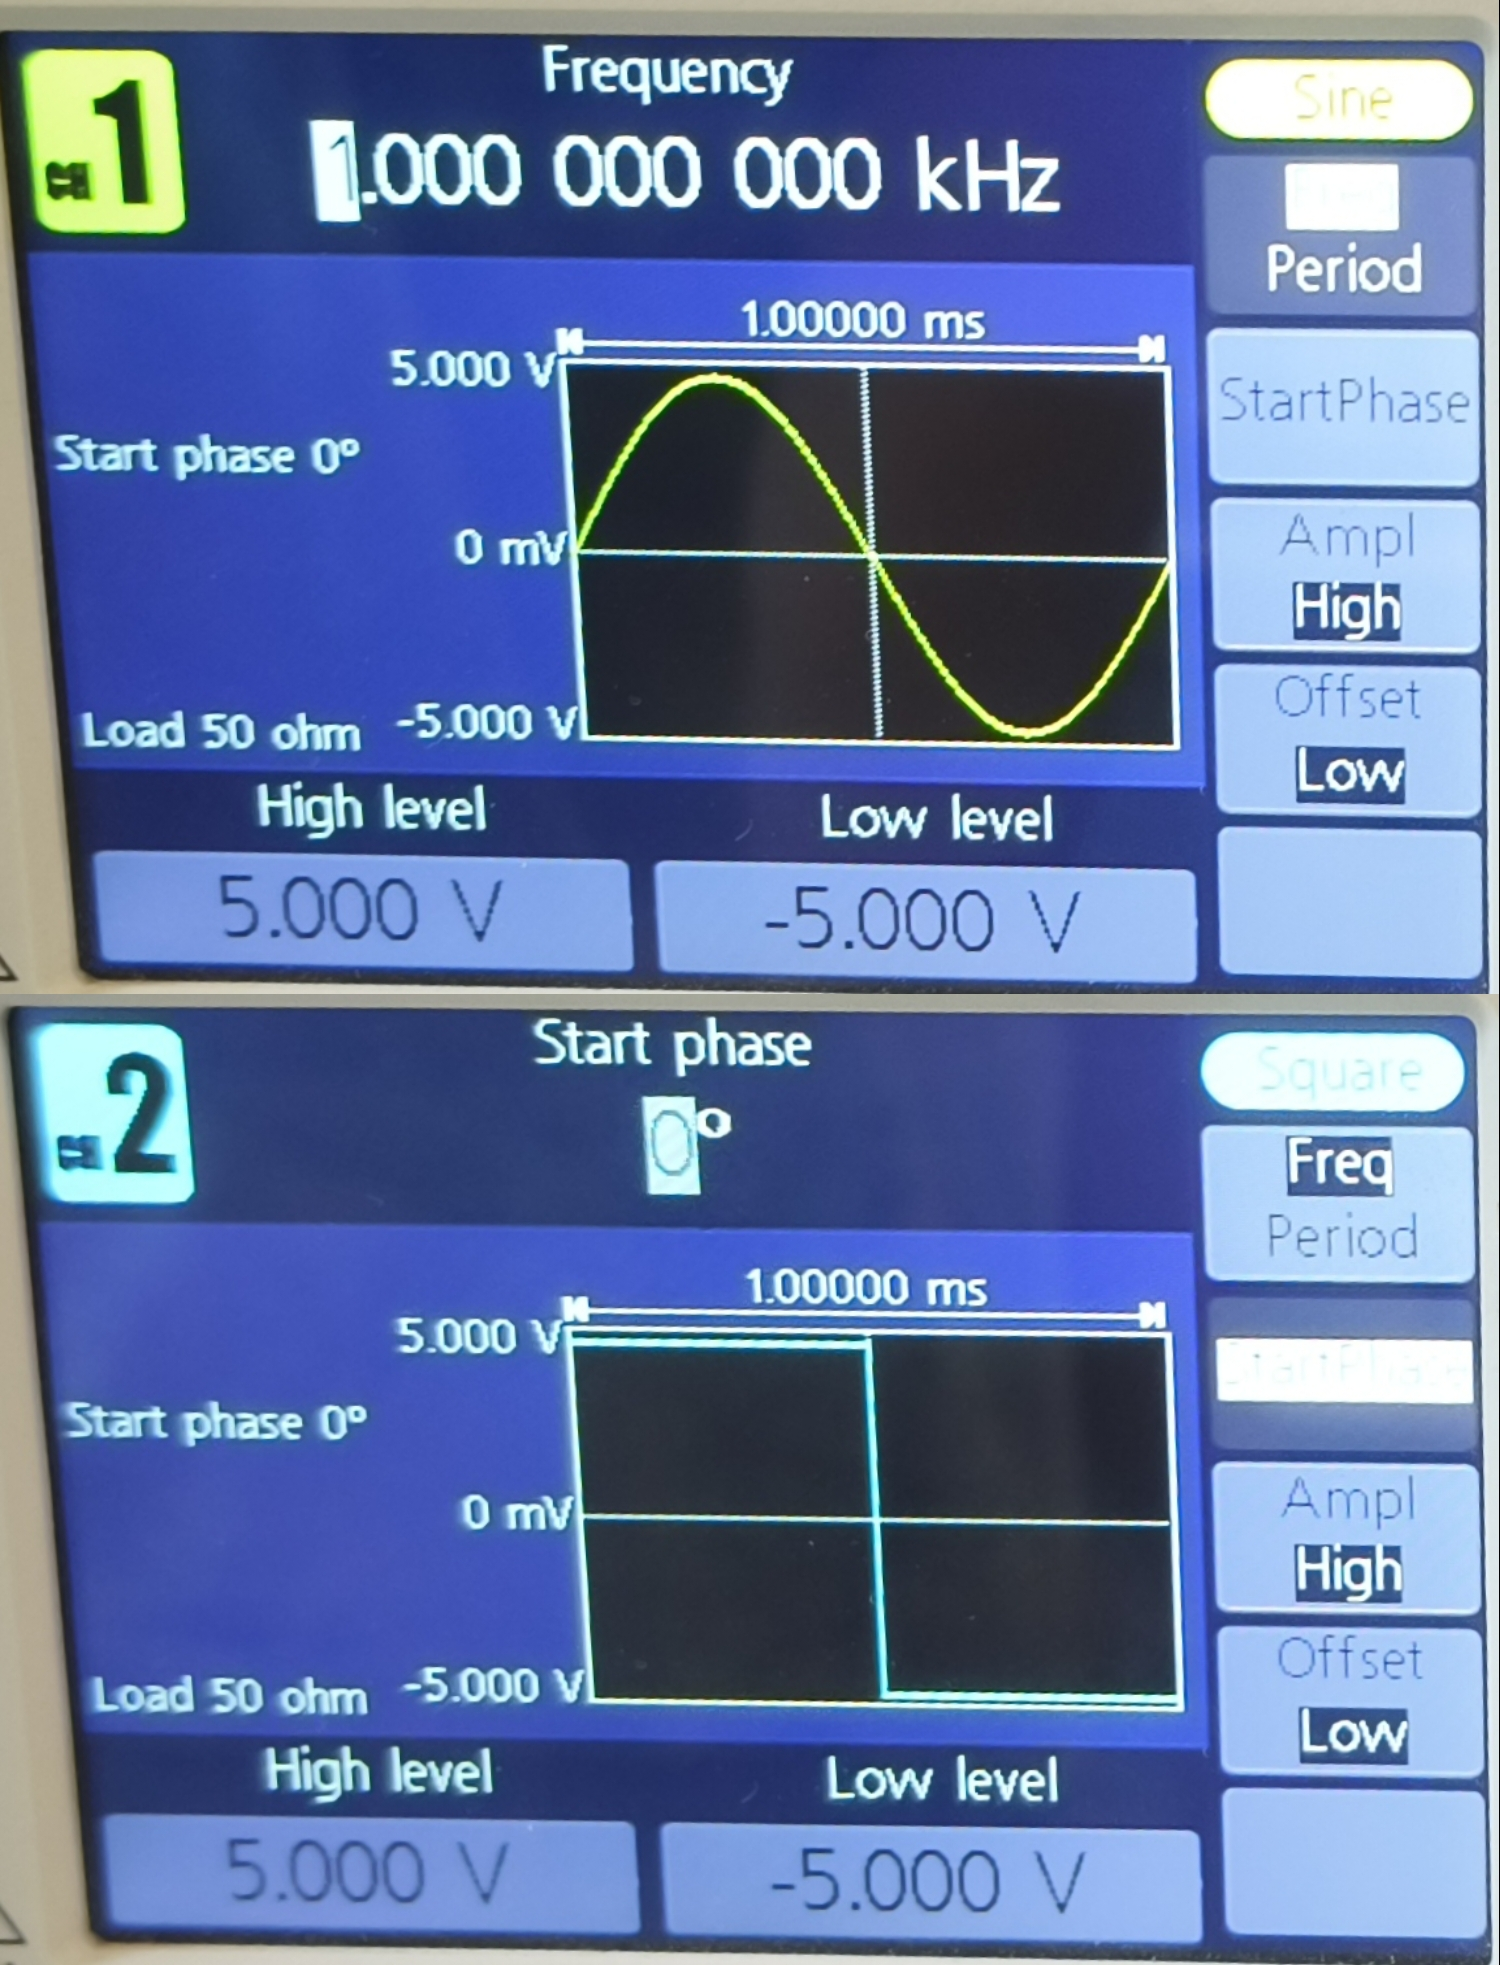
\includegraphics[width=\textwidth]{figs/6read.jpg} % Replace with the actual file name
        
    \end{minipage}
    \hfill
    \begin{minipage}[c]{0.48\textwidth}
        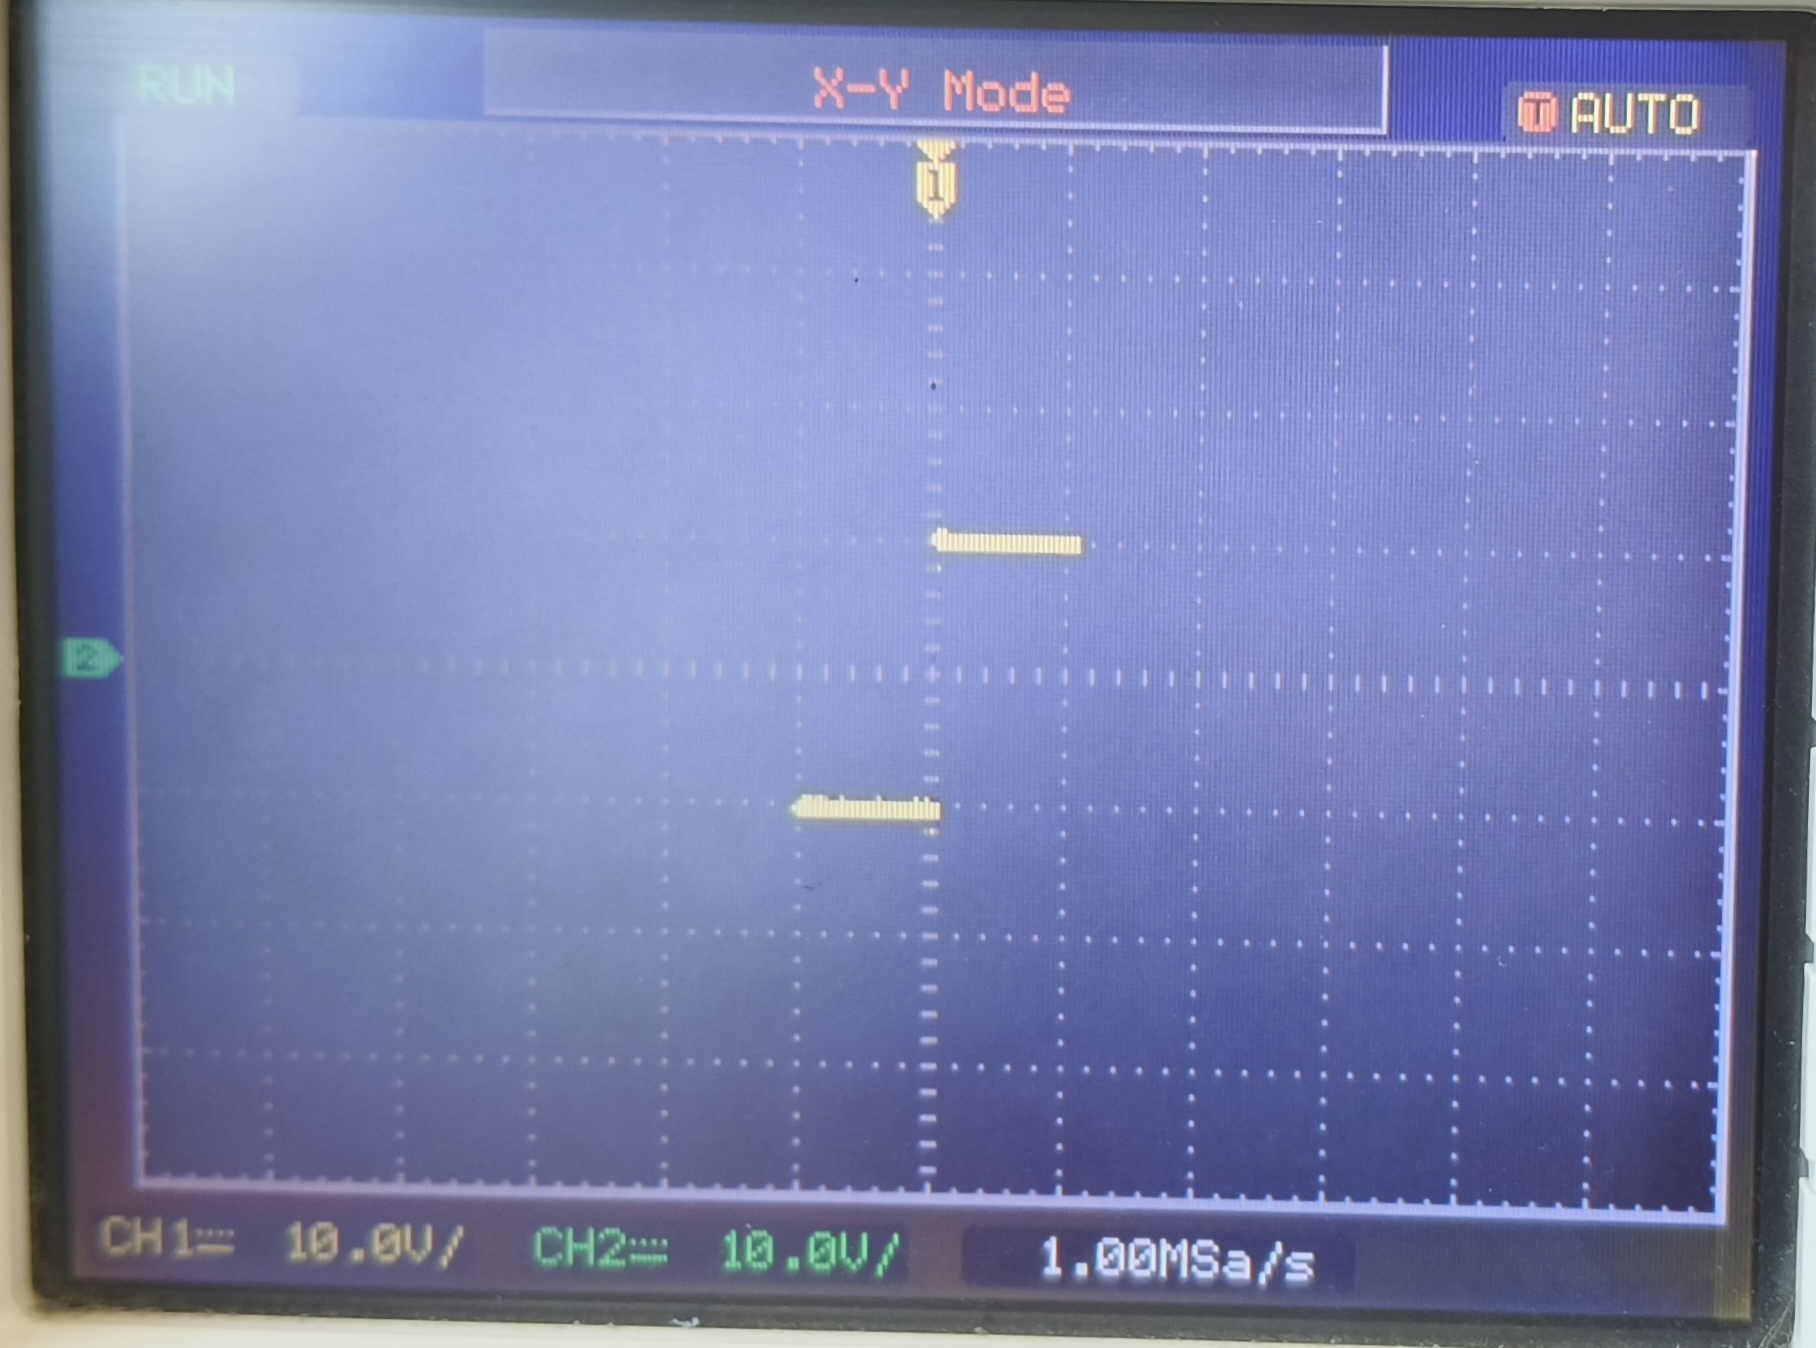
\includegraphics[width=\textwidth]{figs/6cro.jpg} % Replace with the actual file name
        
    \end{minipage}
    \caption{Graph 6}
    \label{fig:CRO-patterns}
\end{figure}

\chapter{One Time Event Capture}
\section{Set Up}
Capture a one-time event using a Cathode Ray Oscilloscope (CRO) and Function Generator.

\section*{Function Generator Configuration}
\begin{enumerate}[leftmargin=*]
    \item Select Burst Mode
    \item Set number of cycles: 5-6 cycles
    \item Configure trigger source to Manual
    \item Adjust amplitude
    \item Set pulse width: 10-50 µs
    \item Wait for manual trigger
\end{enumerate}

\section*{Oscilloscope Configuration}
\begin{enumerate}[leftmargin=*]
    \item Set trigger mode to Normal
    \item Configure trigger to Rising Edge
    \begin{itemize}[leftmargin=*]
        \item Select positive slope trigger
        \item Set trigger level at 50\% of signal amplitude
    \end{itemize}
    \item Select DC coupling
    \item Set vertical sensitivity: 1-2V/div
    \item Adjust time base: 10-20 µs/div
    \item Enable single-shot capture mode
    \item Prepare for manual trigger input
\end{enumerate}

\section*{Experimental Procedure}
\begin{enumerate}[leftmargin=*]
    \item Connect function generator output to oscilloscope input
    \item Verify rising edge trigger settings
    \item Press manual trigger on function generator
    \item Capture single burst event
    \item Save waveform for analysis
\end{enumerate}

\section*{Trigger Specifications}
\begin{itemize}[leftmargin=*]
    \item Oscilloscope Trigger: Rising Edge
    \item Trigger Mode: Normal
    \item Coupling: DC
\end{itemize}
\section*{Observation}
\begin{enumerate}
    \item After setting Normal Mode in oscilloscope it will wait for signal.
    \item  As soon as you press the trigger in Function Generator the oscilloscope captures the signal depending upon mode of rising edge or falling edge.
\end{enumerate}
\subsubsection*{One Time Event Capture}
\begin{figure}[H] % H forces the figure to be placed exactly here
    \centering
    % Replace "1.jpg" with your actual image filename
    \begin{minipage}[c]{0.48\textwidth}
        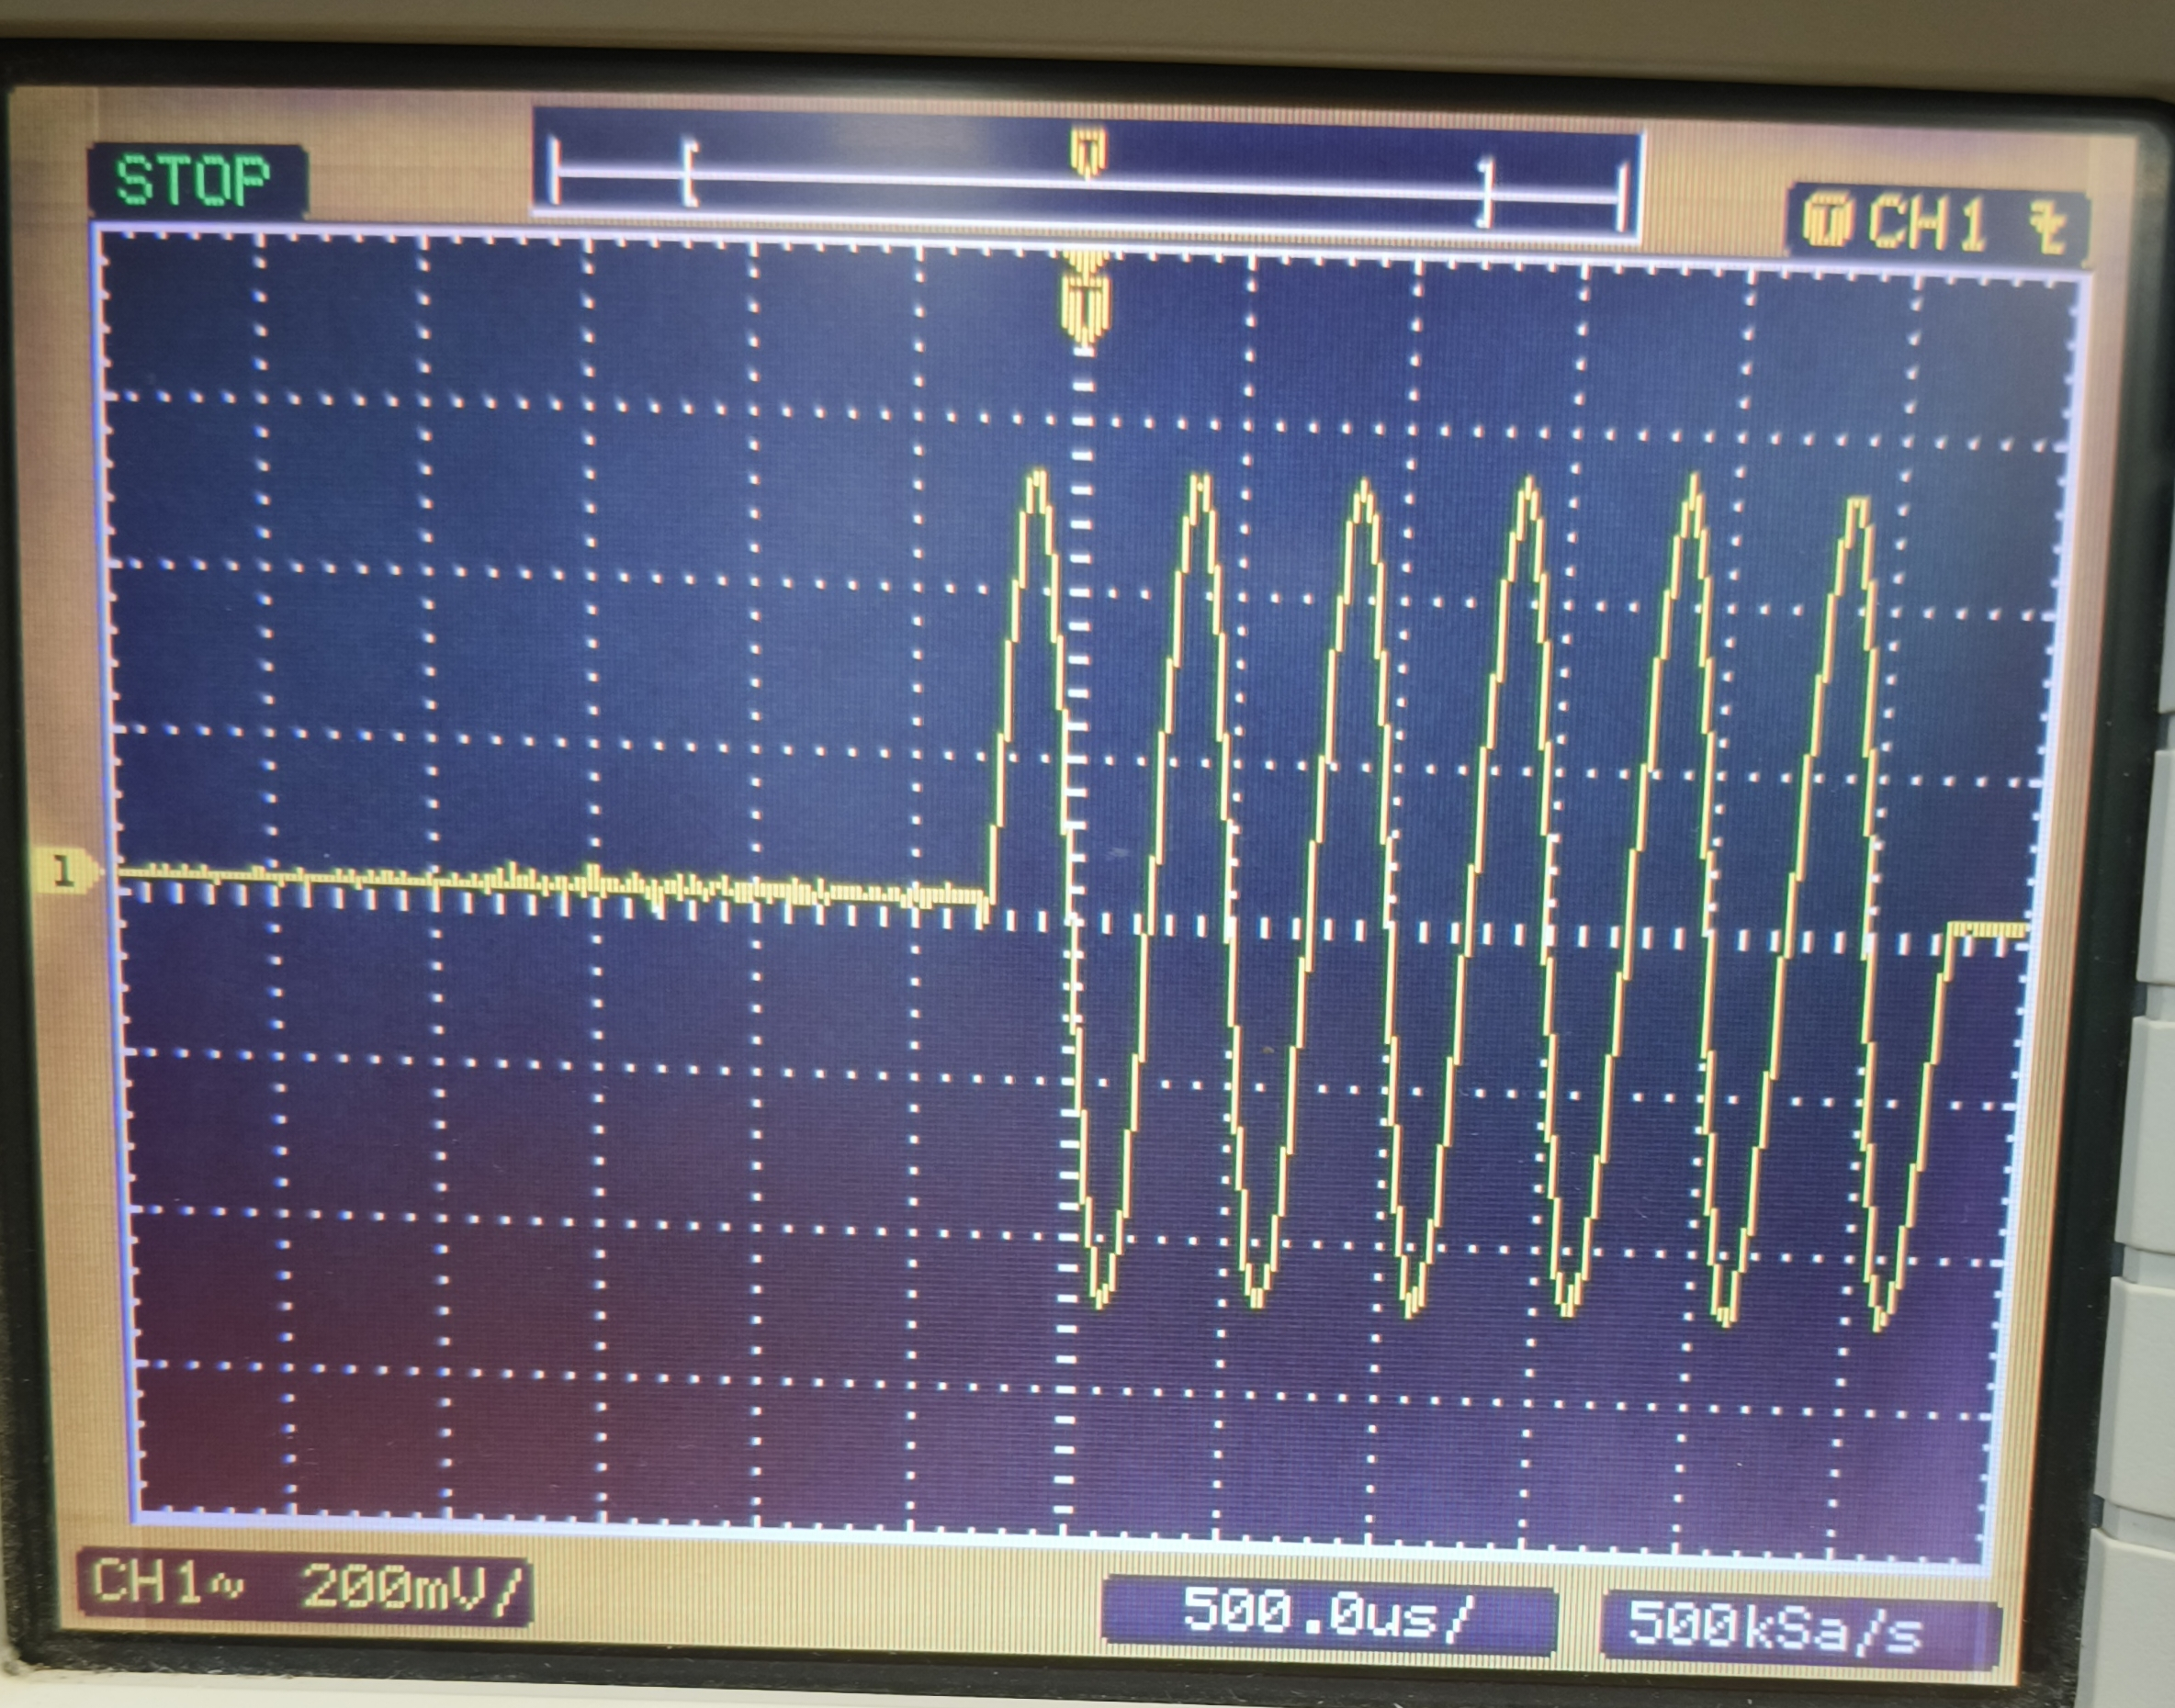
\includegraphics[width=\textwidth]{figs/1cro one.jpg} % Replace with the actual file name
        
    \end{minipage}
    \hfill
    \begin{minipage}[c]{0.48\textwidth}
        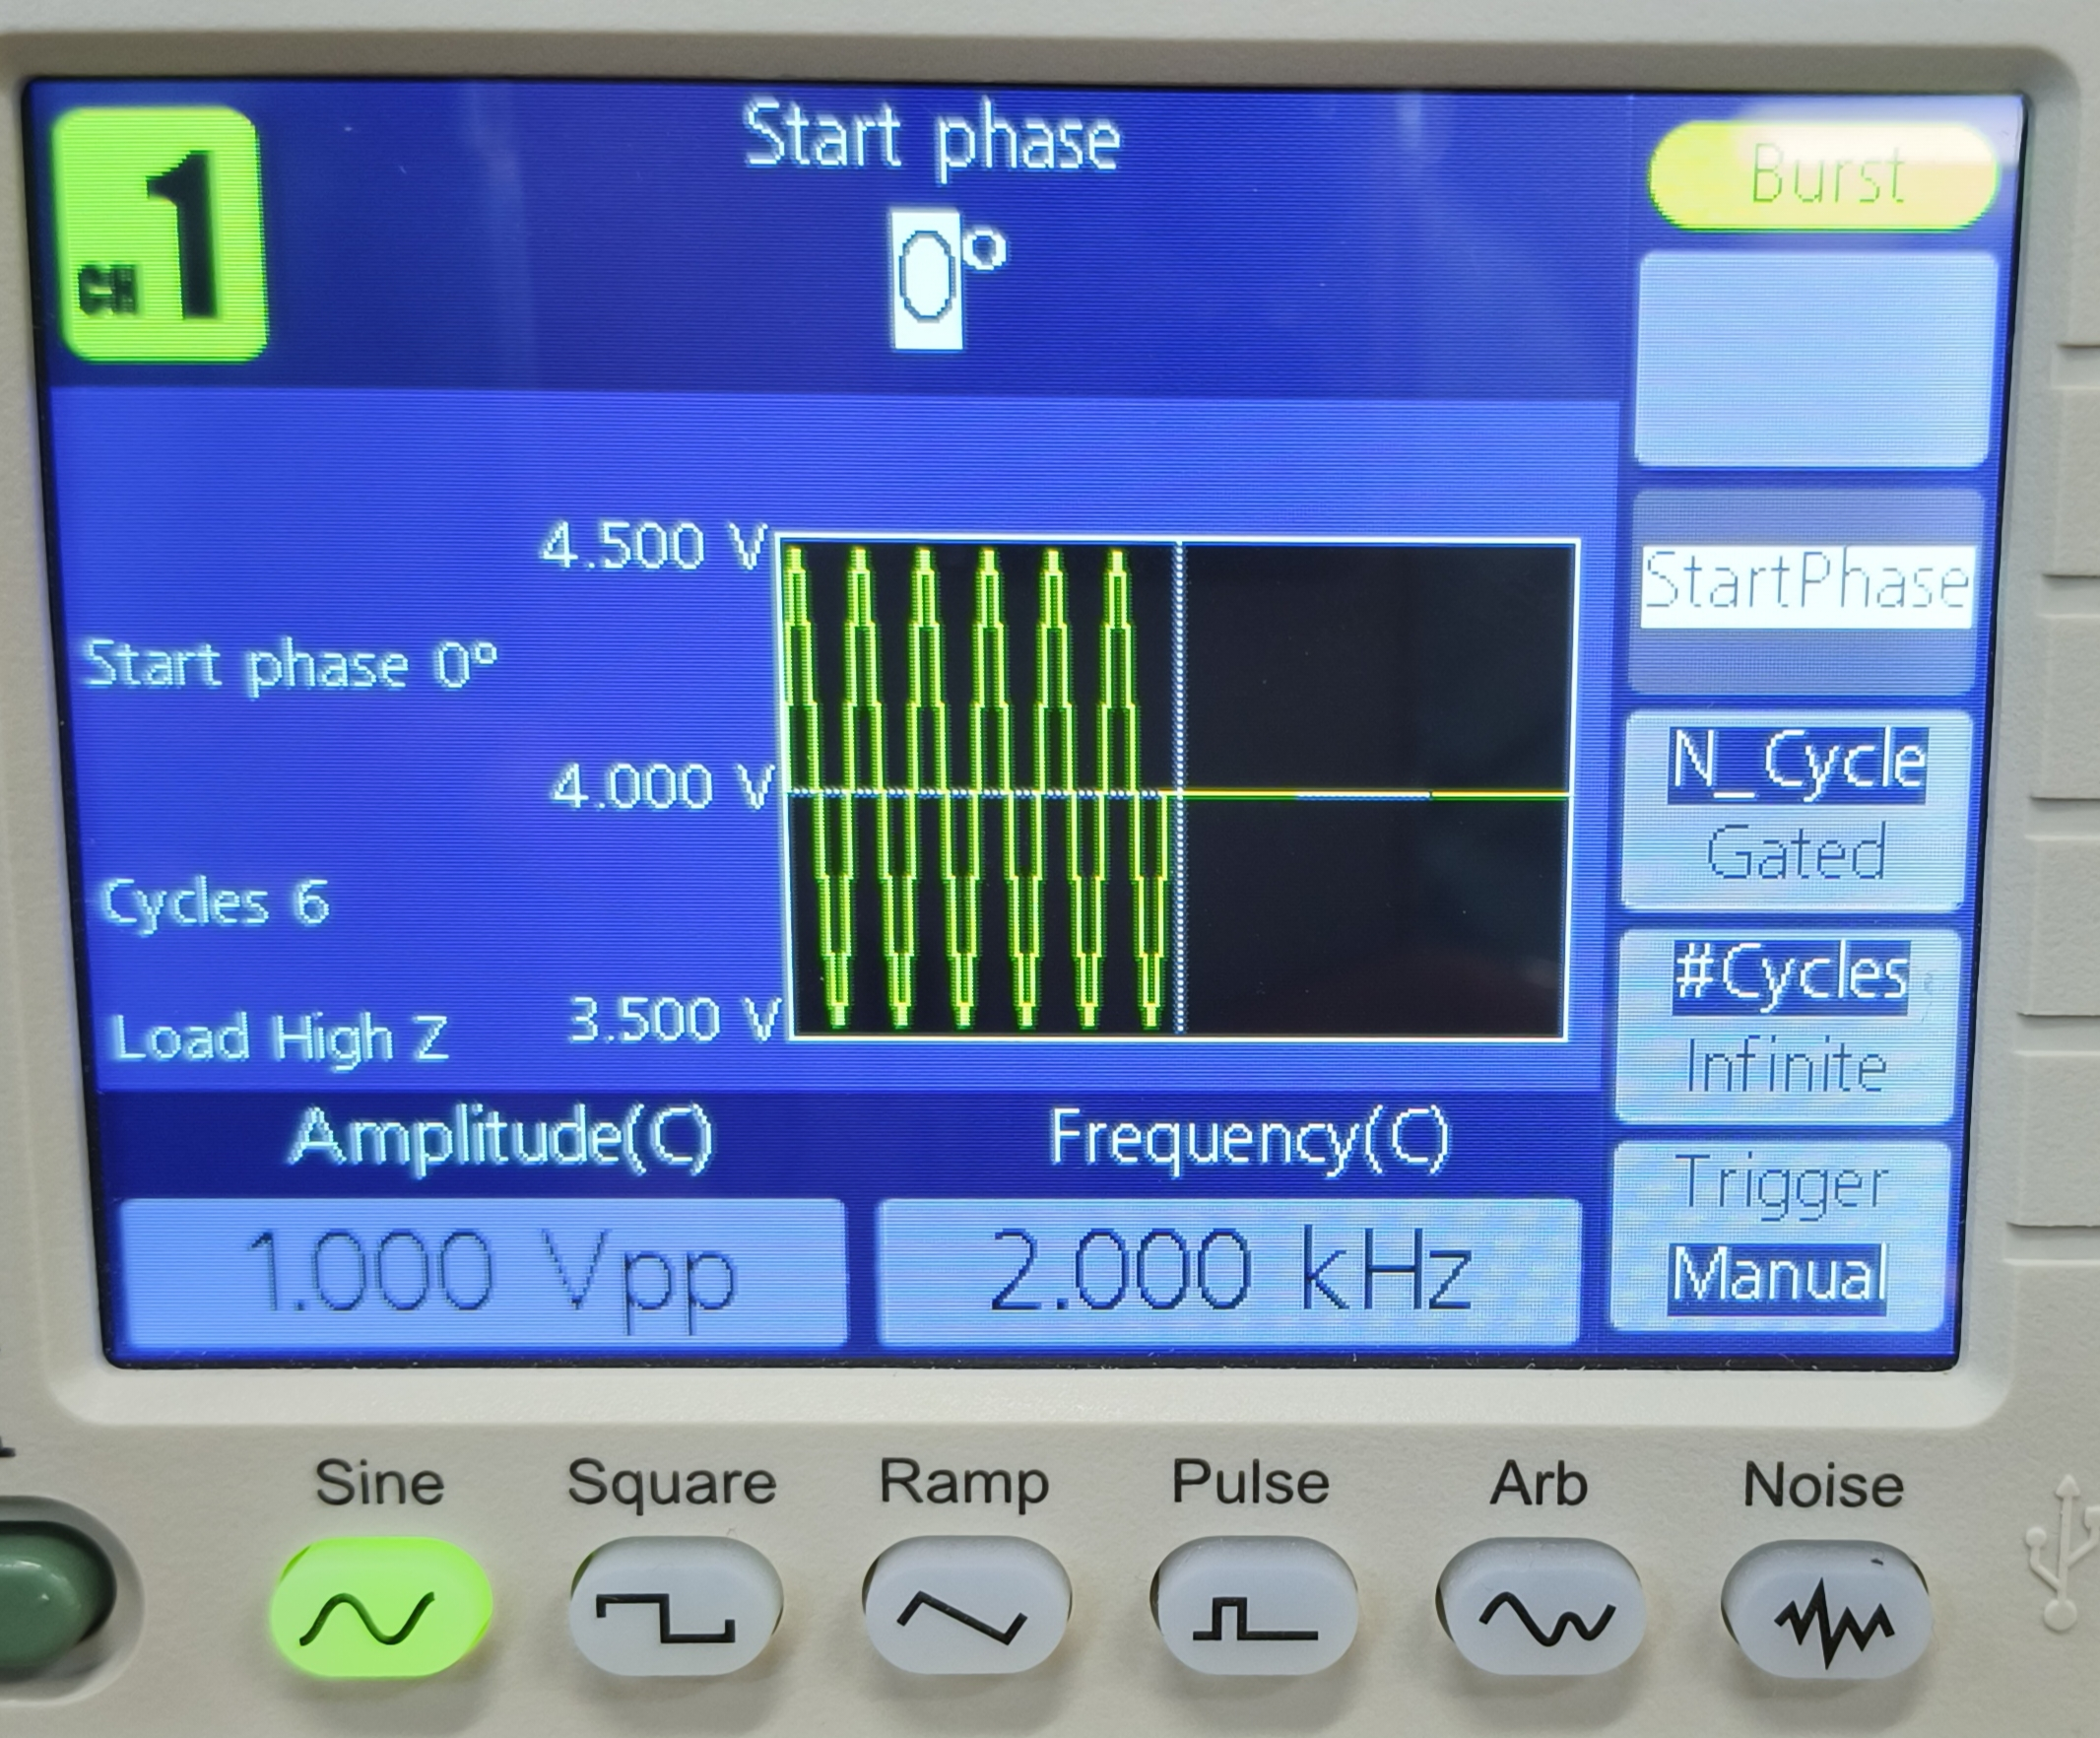
\includegraphics[width=\textwidth]{figs/1one.jpg} % Replace with the actual file name
        
    \end{minipage}
    \caption{One Time Event Graph-1}
    \label{fig:ONE TIME EVENT}
    \end{figure}
    \begin{figure}[H] % H forces the figure to be placed exactly here
    \centering
    % Replace "1.jpg" with your actual image filename
    \begin{minipage}[c]{0.48\textwidth}
        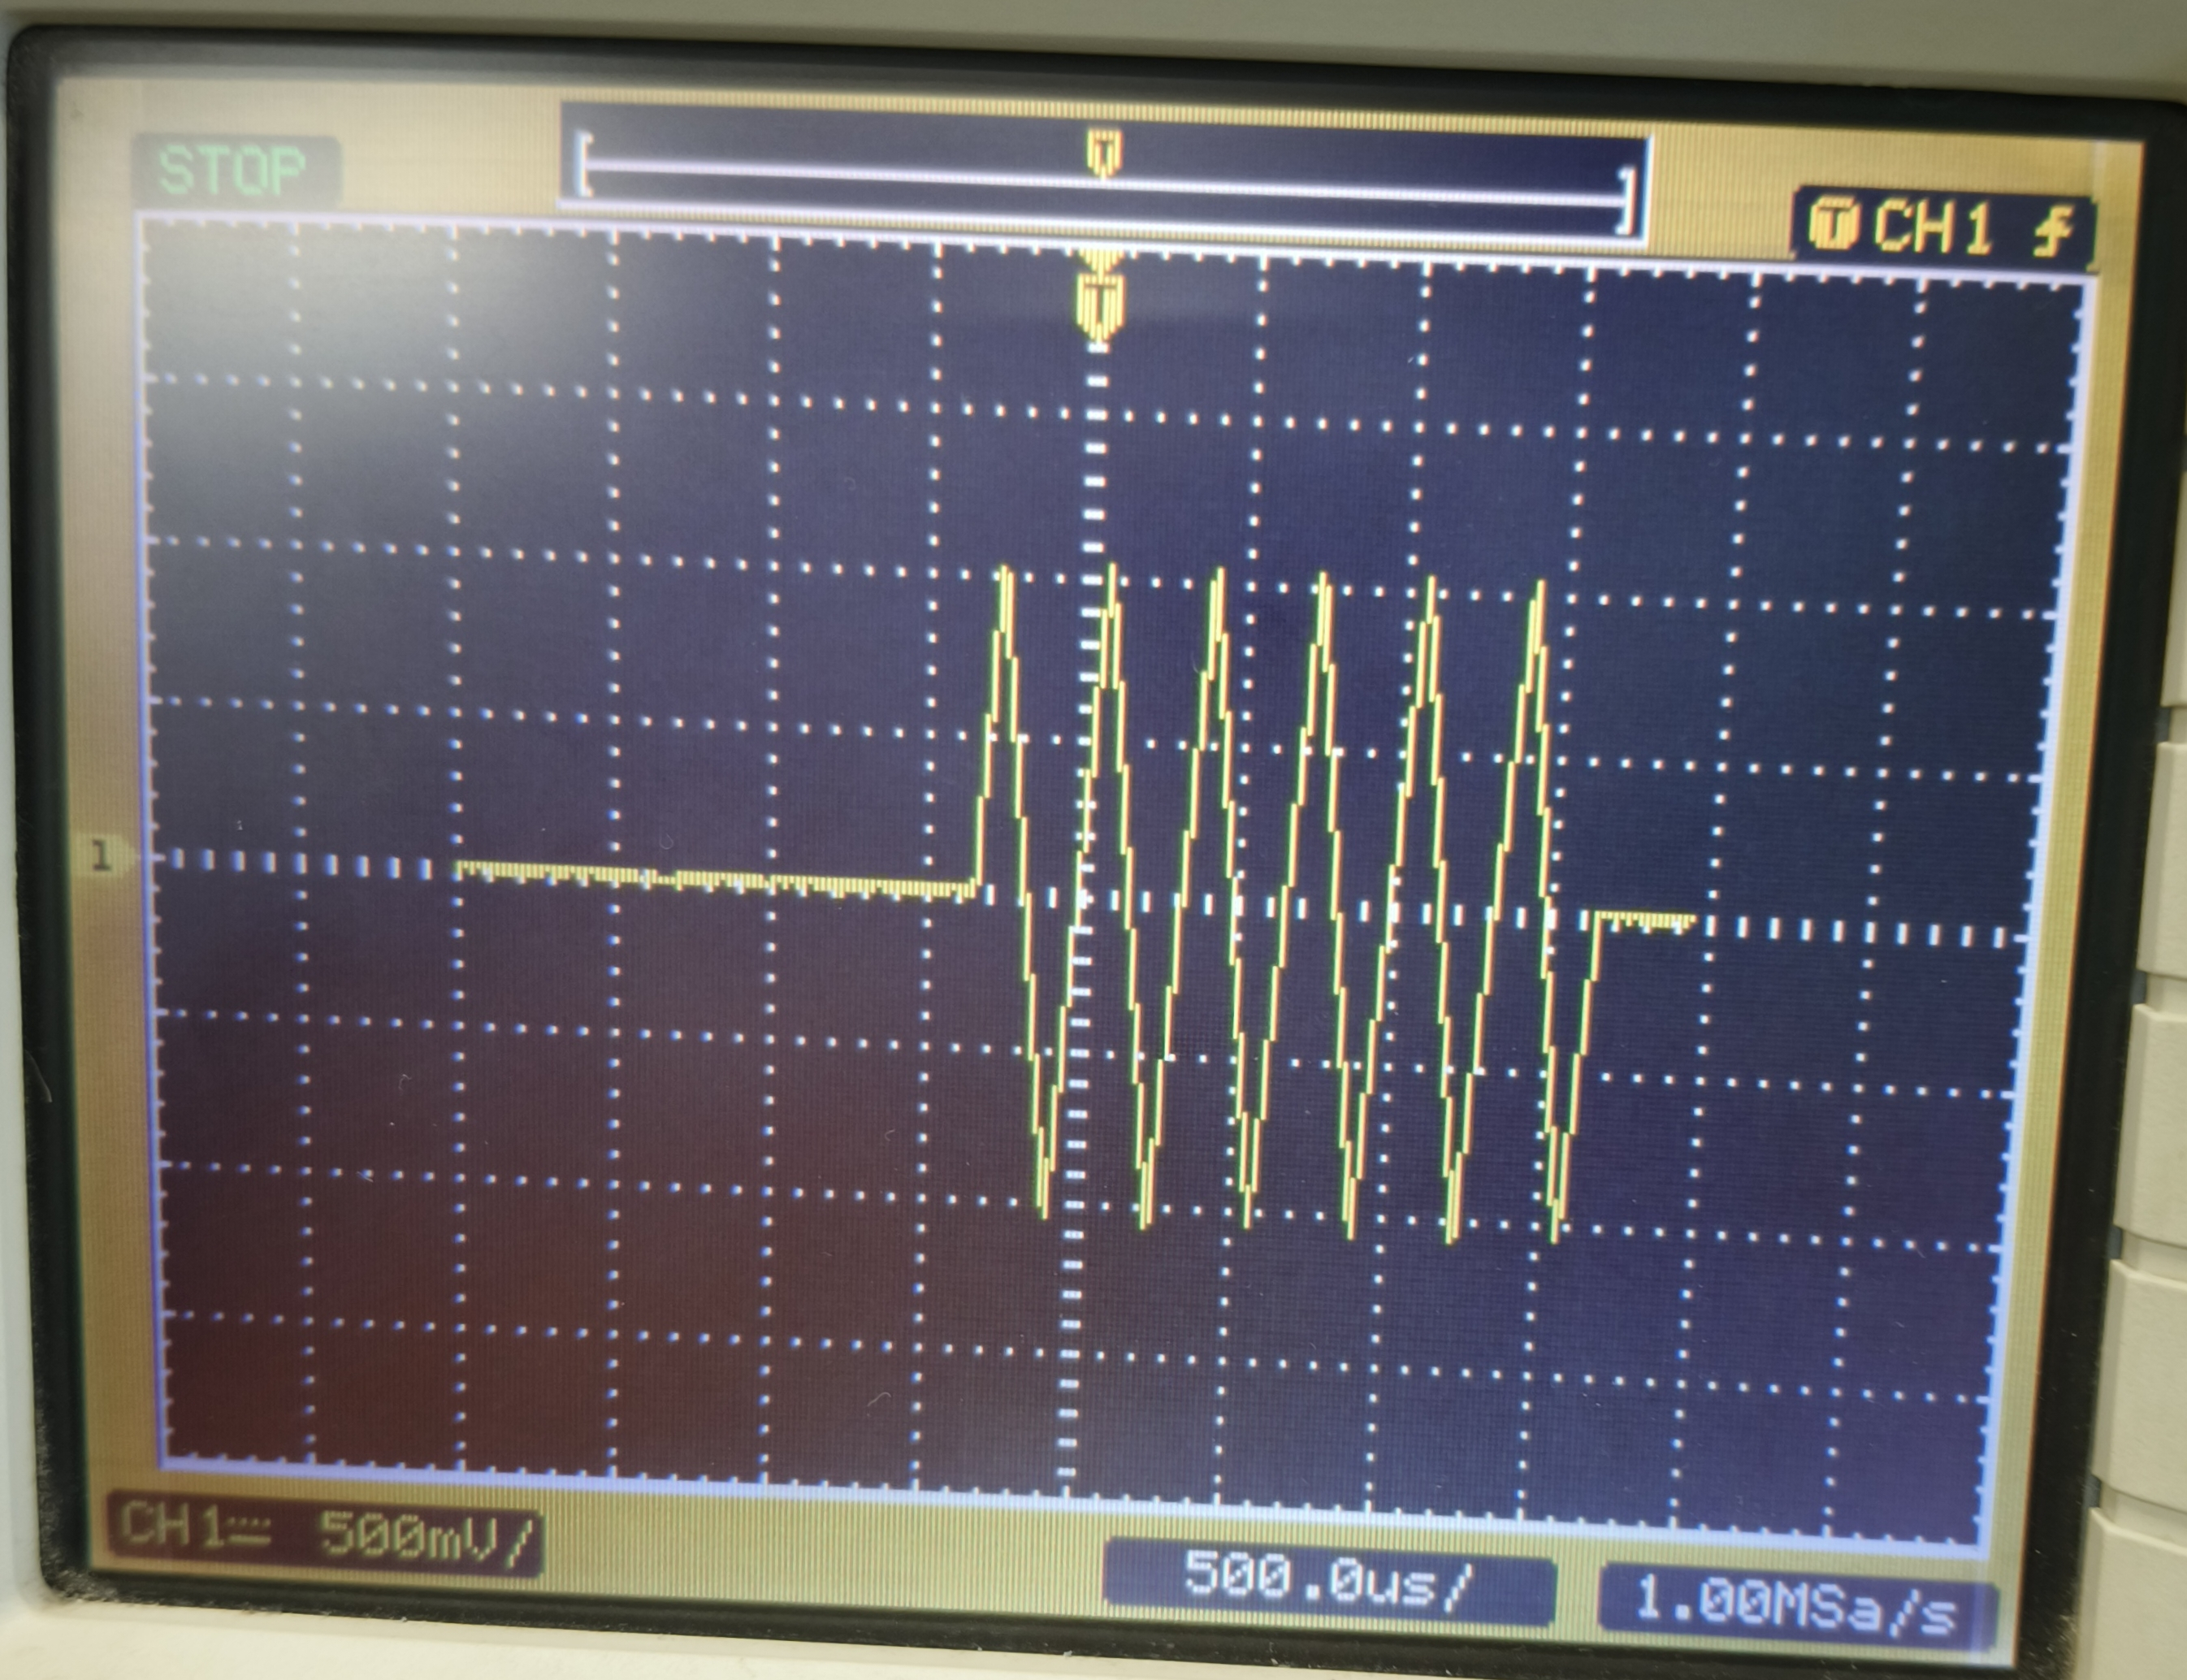
\includegraphics[width=\textwidth]{figs/2cro one.jpg} % Replace with the actual file name
        
    \end{minipage}
    \hfill
    \begin{minipage}[c]{0.48\textwidth}
        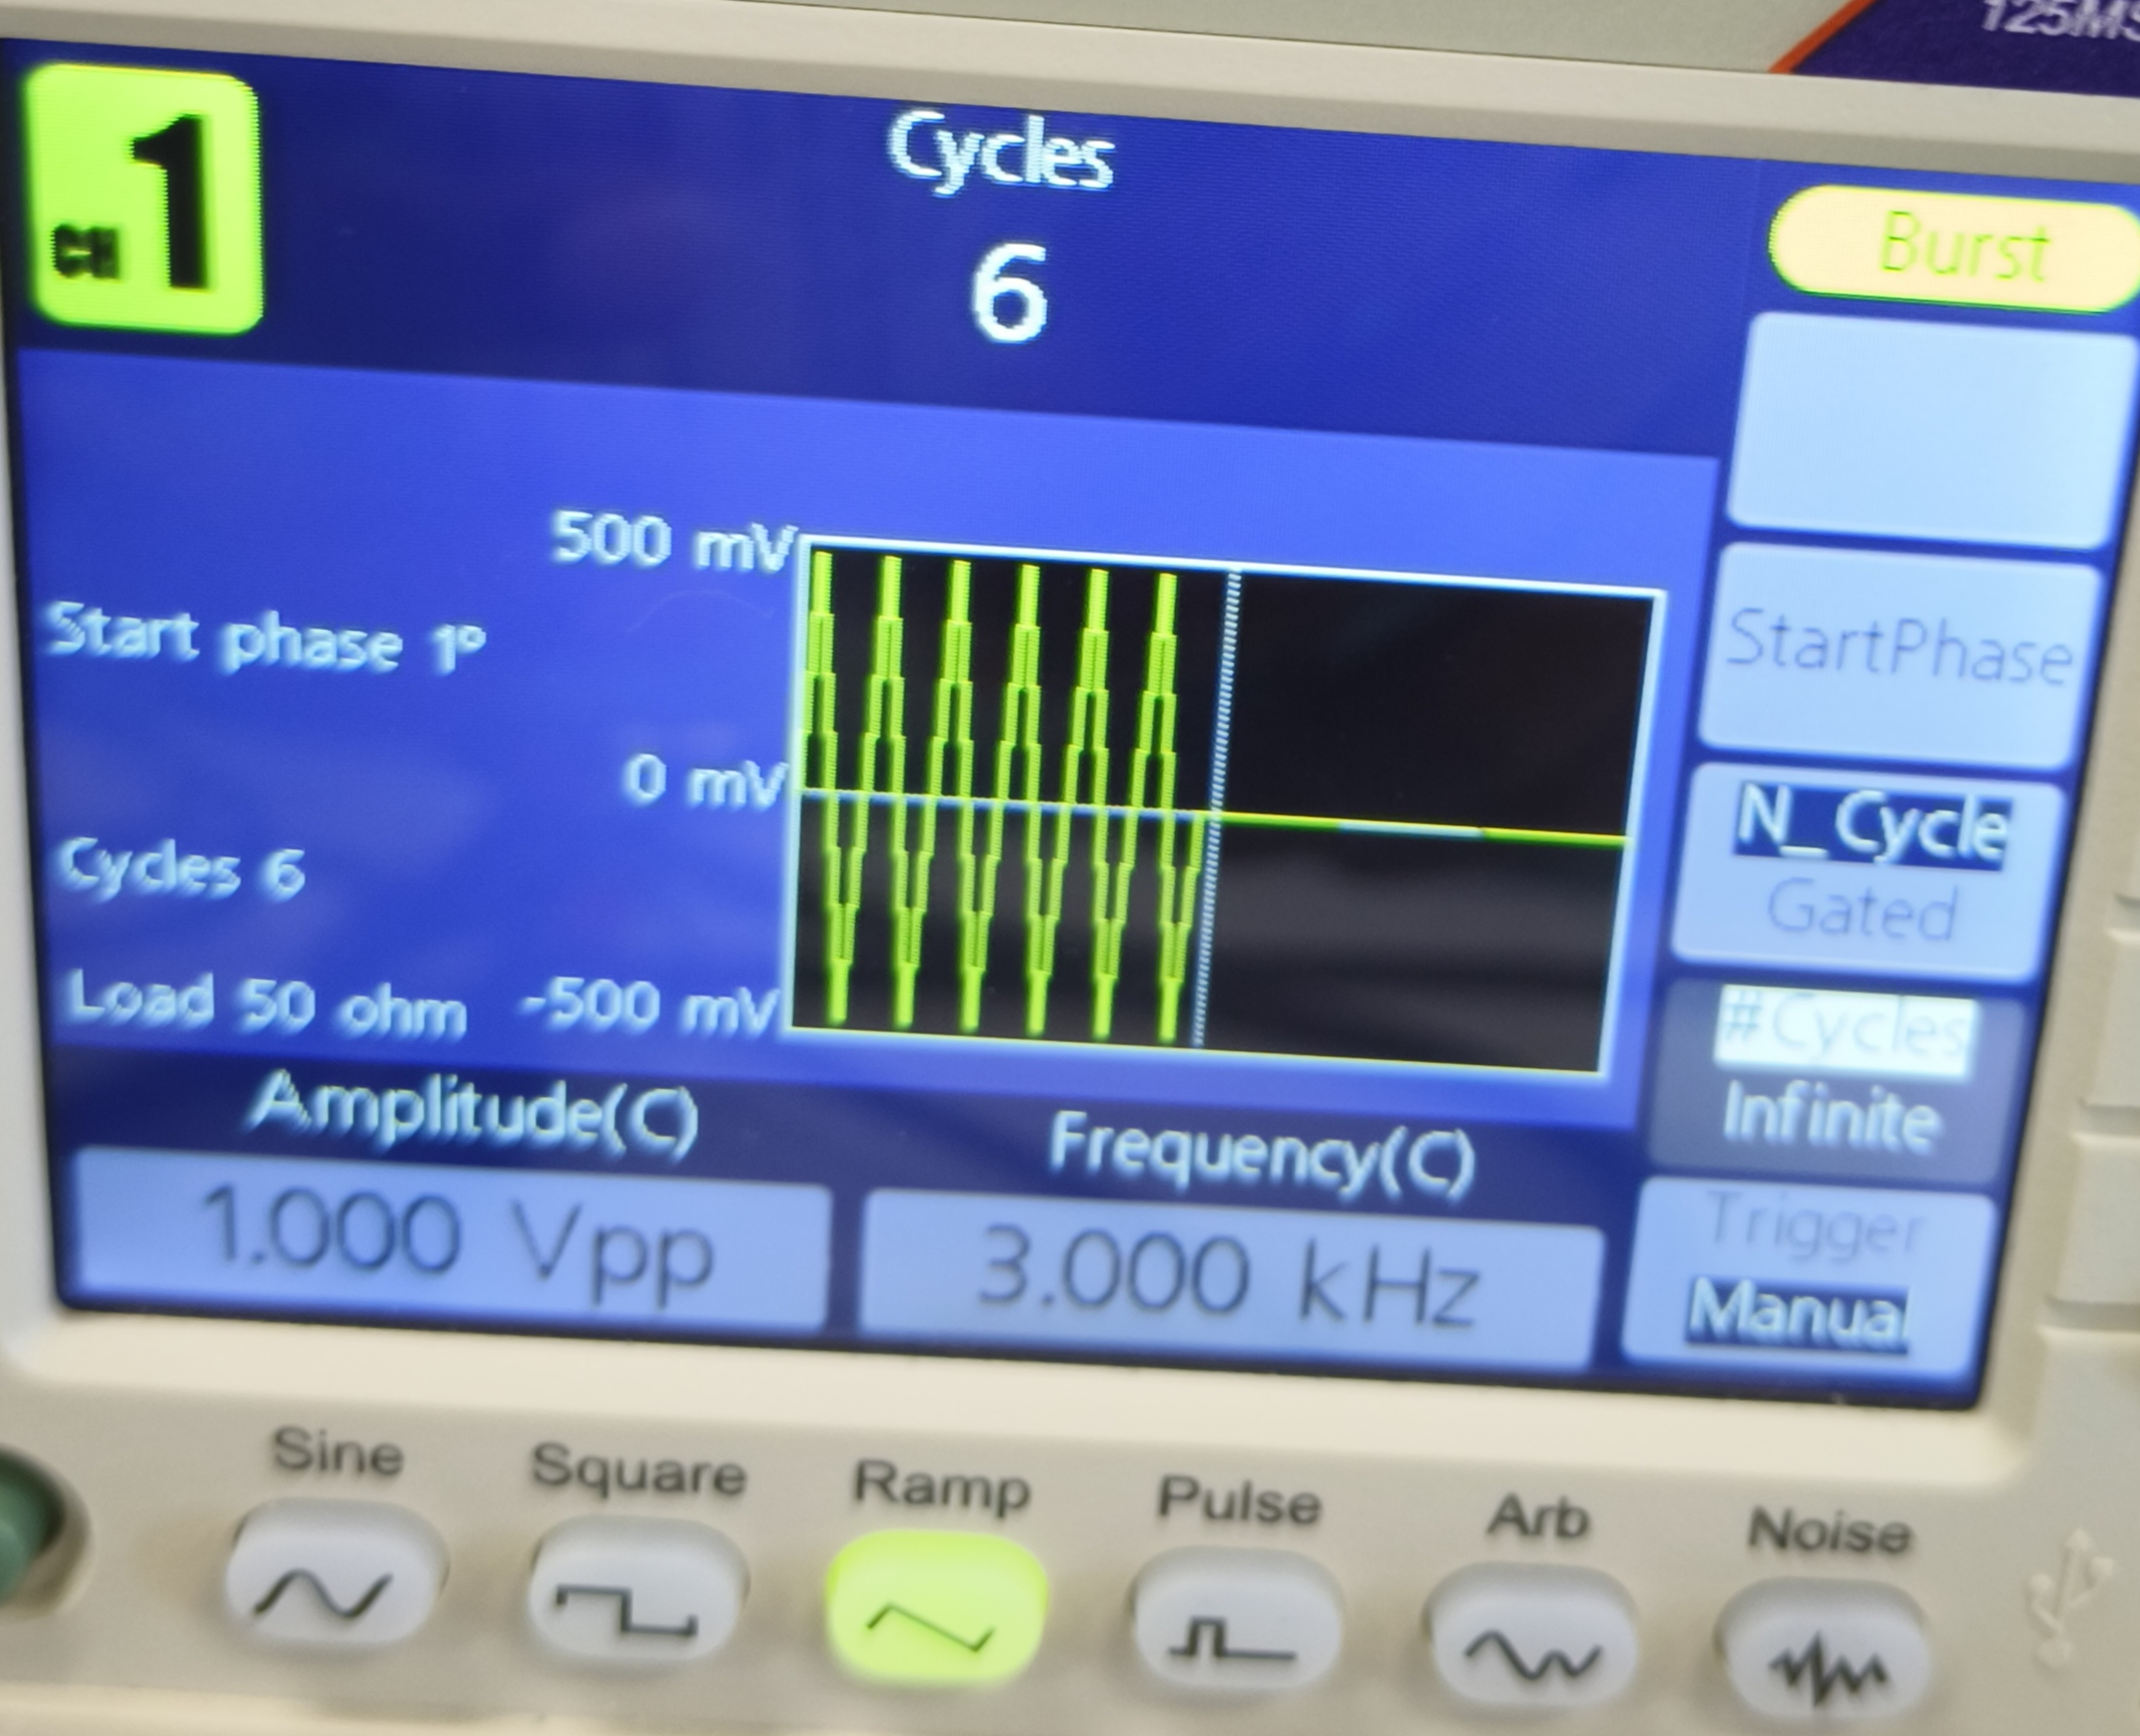
\includegraphics[width=\textwidth]{figs/2one.jpg} % Replace with the actual file name
       
    \end{minipage}
     \caption{One Time Event Graph-2}
    \label{fig:ONE TIME EVENT}
    
\end{figure}
\end{document}
